\documentclass[12pt, a4paper]{report}
\usepackage[utf8]{inputenc}
\usepackage[T5]{fontenc}
\usepackage[english]{babel}
\usepackage{minted}
\usepackage{graphicx}
\usepackage{caption}
\usepackage{geometry}
\usepackage{hyperref}
\usepackage{amsmath}
\usepackage{float}
\usepackage{booktabs}
\usepackage{longtable}
\usepackage{array}
\usepackage{multicol}
\usepackage{pdflscape}
\usepackage{setspace}
\usepackage{background}
\usepackage{natbib}
\usepackage{enumitem} 

\backgroundsetup{
    scale=1,
    color=black,
    opacity=1,
    angle=0,
    position=current page.center,
    contents={
\includegraphics[width=\paperwidth,height=\paperheight]{background.png}}
}

\hypersetup{
    colorlinks=true,
    linkcolor=black,
    citecolor=black,
    urlcolor=black
}

\geometry{a4paper, margin=1in}

\begin{document}

\begin{titlepage}
\BgThispage
    \centering
    \textbf{\large POSTS AND TELECOMMUNICATIONS INSTITUTE OF TECHNOLOGY}\\
    \textbf{\large FACULTY OF INFORMATION TECHNOLOGY I}
    \centerline{--------------------o0o--------------------}
    \vspace{1cm}
    
\includegraphics[width=8cm]{logo.png}\\ 
    \vspace{1cm}
{\Large \textbf{ASSIGNMENT REPORT 1}}\\[0.5cm]
{\LARGE \textbf{PYTHON PROGRAMMING LANGUAGE}}\\
\vfill
\begin{center}
\begin{tabular}{@{}l@{\hspace{2cm}}l}
\textbf{Instructor:}       & Kim Ngoc Bach \\
\textbf{Student:}          & Vu Thi Thu Duyen \\
\textbf{Student ID:}       & B23DCCE027 \\
\textbf{Class:}            & D23CQCEO6-B \\
\textbf{Academic Year:}    & 2023 - 2028 \\
\textbf{Training System:}  & Full-time University \\
\end{tabular}
\end{center}
\vfill
    {\large Hanoi, 2025}
\end{titlepage}
\backgroundsetup{contents={}}

\newgeometry{top=2.5cm,bottom=2cm,left=3cm,right=2cm}

\begin{center}
	{\textbf{\Large{LECTURER'S COMMENTS }}}
\end{center}

\dotfill \vspace{0.25cm} \par
\dotfill \vspace{0.25cm} \par
\dotfill \vspace{0.25cm} \par
\dotfill \vspace{0.25cm} \par
\dotfill \vspace{0.25cm} \par
\dotfill \vspace{0.25cm} \par
\dotfill \vspace{0.25cm} \par
\dotfill \vspace{0.25cm} \par
\dotfill \vspace{0.25cm} \par
\dotfill \vspace{0.25cm} \par
\dotfill \vspace{0.25cm} \par
\dotfill \vspace{0.25cm} \par
\dotfill \vspace{0.25cm} \par
\dotfill \vspace{0.25cm} \par
\dotfill \vspace{0.25cm} \par
\dotfill \vspace{0.25cm} \par
\dotfill \vspace{0.25cm} \par
\dotfill \vspace{0.25cm} \par
\dotfill
\vspace{1cm}

{\textbf{\large{Score: }}} \hspace{1.0cm}\textbf{( In words:}  \hspace{2.5cm}\textbf{)} 



\begin{flushright}
	Hanoi, date \hspace{0.75cm} month \hspace{0.75cm} year 20...\hspace{0.75cm}
	
	{\textbf{\large{Lecturer  }}} \hspace{2cm} \textcolor{white}{.}
\end{flushright}
\clearpage
\tableofcontents
\newpage
\listoffigures
\newpage

\chapter{Collecting English Premier League Player Statistics for the 2024-2025 Season from \href{http://fbref.com}{fbref.com}}
\author{}
\date{}

% Chương 1
\section{Introduction}
This exercise requires building a Python program to automatically collect detailed statistical data of football players in the English Premier League (EPL) for the 2024-2025 season from the website \texttt{fbref.com}.
The program will generate two output files:
\begin{itemize}
\renewcommand{\labelitemi}{}
    \item \texttt{results.csv}: Contains data of players whose total minutes played throughout the season (for one or more clubs) exceed 90 minutes, as per the specific requirement of this exercise.
    \item \texttt{results1.csv}: Contains data of players who played more than 90 minutes for a specific club during the season. This file retains individual records per team and will be crucial input data for subsequent statistical analysis and aggregation exercises that require detailed data per club appearance of the player.
\end{itemize}
The following sections will describe the implementation process, including library selection, the data scraping workflow, and the obtained results.

\section{Library Selection}
To perform the task of scraping data from a dynamic website and processing the data efficiently, the following Python libraries were selected:
\begin{itemize}
\renewcommand{\labelitemi}{}
    \item \textbf{Selenium}: This library was chosen as the primary tool for interacting with the FBRef website because this site heavily uses JavaScript to load and display content, especially complex statistical tables. Unlike the \texttt{requests} library (which only fetches the initial static HTML source code sent by the server and cannot execute JavaScript), \texttt{selenium} operates by controlling a real web browser (like Chrome or Firefox) automatically. This allows the script to wait for dynamic elements (such as data tables) to be fully loaded and displayed by JavaScript, execute any JavaScript code on the page, and access the final, completely rendered HTML structure (DOM). Using only \texttt{requests} would carry a high risk of missing important data tables or receiving incomplete data, as they are generated or populated by JavaScript after the initial page load.
    \item \textbf{BeautifulSoup4 (bs4)}: After \texttt{selenium} finishes loading the page and retrieves the HTML source code, \texttt{BeautifulSoup} is used to parse that HTML. It provides convenient methods for navigating HTML, finding specific tags and attributes (such as \texttt{id}, \texttt{class}, \texttt{data-stat}), and extracting text content easily and efficiently.
    \item \textbf{Pandas}: This is a powerful library for data manipulation and analysis.
    \item \textbf{Json}: The \texttt{config.json} file contains important configurations such as the base URL, names of the statistics to retrieve, corresponding data table IDs, \texttt{data-stat} attributes, minimum minutes threshold, etc. The \texttt{json} library is used to read and parse this configuration file, making the main source code cleaner, more readable, and easier to maintain. Separating the configuration makes it easy to change parameters or update for website structure changes without significant modifications to the Python script.
    \item \textbf{Re (Regular Expressions)}: Used to extract the unique player ID from URL paths in the HTML code (\texttt{/players/<player\_id>/}). This ID is crucial for identifying and aggregating data for the same player when they appear in multiple statistical tables or play for multiple clubs within a season.
    \item \textbf{Time}: Used to introduce small delays (\texttt{time.sleep}) between web page access requests, to avoid sending too many consecutive requests to the FBRef server, reducing the risk of IP blocking and demonstrating "polite" web Browse behavior.
    \item \textbf{Collections.defaultdict}: Extremely useful when aggregating data. In cases where a player plays for multiple clubs in the same season (e.g., a mid-season transfer), they will appear multiple times in the data table. \texttt{defaultdict} is used to create a data structure that allows summing the minutes played (\texttt{Min}) for that player from different rows before applying the minimum minutes filter.
\end{itemize}

\section{Web Scraping Process}
The main idea of this script is to automate the process of collecting data from a dynamic web source (fbref.com) by combining Selenium to simulate user behavior and BeautifulSoup to parse the HTML structure. The data to be retrieved is determined by an external configuration (\texttt{config.json}), allowing for flexible selection of necessary statistics from various tables on the page.
A key aspect of data processing is that the program initially identifies each individual statistical record by a pair (unique player ID or name, team name). This is necessary to accurately distinguish the data of the same player when they play for different clubs within the same season (e.g., after a transfer), because on fbref, a player can appear in multiple rows if they change teams.
Subsequently, this data is processed in two distinct ways to generate two CSV files:
\begin{itemize}
    \item \textbf{results1.csv}: Directly filtered from the detailed data, retaining records where the player played > 90 minutes for that specific club.
    \item \textbf{results.csv}: Aggregates the total minutes played for each player across the entire season, then filters for players whose total minutes exceed 90, and outputs all records related to that player (including records with less than 90 minutes for a specific club, as long as the total minutes meet the requirement).
\end{itemize}
\textbf{The web scraping process is carried out in the following steps:}
\begin{enumerate}[label=\textbf{Step \arabic*:}, leftmargin=*]
    \item \textbf{Load Configuration}: The program begins by reading the \texttt{config.json} file to obtain necessary information such as the base URL for the EPL season on fbref, the list of statistical metrics to collect, IDs of the HTML tables containing the data, the \texttt{data-stat} attribute corresponding to each metric, the minimum playing time threshold (\texttt{min\_minutes}), output CSV filenames, and the column order for the result files.
    \item \textbf{Initialize Selenium}: An automated web browser (WebDriver) is initialized using \texttt{selenium}.
    \item \textbf{Access and Load Page}:
    \begin{itemize}[leftmargin=0em]
        \item The program navigates to the URL of the main statistics table (\texttt{stats}) for the EPL 2024-2025 season.
        \item Uses \texttt{WebDriverWait} to wait until the main data table (\texttt{stats\_standard}) appears and is interactable, ensuring that all data loaded by JavaScript is displayed.
    \end{itemize}
    \item \textbf{Initial HTML Parsing}: The complete HTML source code of the loaded page is retrieved from \texttt{selenium} and passed to \texttt{BeautifulSoup} for parsing.
    \item \textbf{Collect Data from Multiple Tables}:
    \begin{itemize}[leftmargin=0em]
        \item The script is designed to retrieve data from various types of statistical tables on fbref (Standard, Shooting, Passing, Defensive Actions, etc.), as defined in the \texttt{STATS\_CONFIG} section of the \texttt{config.json} file.
        \item For each type of statistic, the script constructs the corresponding URL (e.g., \texttt{.../stats/}, \texttt{.../shooting/}, \texttt{.../passing/}).
        \item The script accesses each of these URLs using \texttt{selenium}, waits for the respective data table to load, retrieves the HTML, and uses \texttt{BeautifulSoup} to parse it.
        \item Iterates through each row (\texttt{<tr>}) in the body (\texttt{<tbody>}) of the data table.
    \end{itemize}
    \item \textbf{Extract Player Data}: For each row (representing a player in that table), the script performs the following:
    \begin{itemize}[leftmargin=0em]
        \item Finds the cell containing the player's name and extracts the name (\texttt{Player}) and the unique player ID (\texttt{player\_id}) from the player profile link using regular expressions (\texttt{re}).
        \item Uses the \texttt{safe\_get\_text} function, \texttt{get\_nation\_code}, and the \texttt{data-stat} configuration from \texttt{config.json} to extract the value of each requested statistical metric for that player.
        \item This function ensures that "N/a" is returned if a data cell does not exist or is empty.
    \end{itemize}
    \item \textbf{Temporary Storage}: The data for each player from each table is stored in a dictionary, which is then added to a consolidated list (\texttt{scraped\_data}).
    \item \textbf{Aggregate and Filter Data (2 flows)}:
    \begin{itemize}[leftmargin=0em]
        \item Flow 1: Create data for \texttt{results1.csv}
        \begin{itemize}
            \item Iterate through \texttt{scraped\_data}.
            \item For each record (corresponding to a player at a specific team), check the value of \texttt{Playing Time: minutes ('Min')}.
            \item If the minutes > \texttt{MIN\_MINUTES}, reformat the values (using \texttt{format\_value}) and add this record's dictionary to the \sloppypar
            \texttt{single\_team\_over\_90\_list} list.
        \end{itemize}
        \item Flow 2: Create data for \texttt{results.csv}
        \begin{itemize}
            \item Use \texttt{collections.defaultdict} (\texttt{player\_minutes\_aggregate}) to group records by \texttt{player\_id} (or \texttt{player\_name} if ID is not available).
            \item During the grouping process, sum the minutes played (\texttt{Min}) to calculate \texttt{total\_minutes} for each player.
            \item Filter \texttt{player\_minutes\_aggregate}, keeping only players with \texttt{total\_minutes} > \texttt{MIN\_MINUTES}.
            \item For each eligible player, iterate through \textit{all} original records (entries) of that player (from different teams if applicable).
            \item Reformat the values for each record and add it to the \sloppypar \texttt{final\_player\_list\_of\_dicts} list.
        \end{itemize}
    \end{itemize}
    \item \textbf{Format and Sort}:
    \begin{itemize}[leftmargin=0em]
        \item Both lists (\texttt{single\_team\_over\_90\_list} and \texttt{final\_player\_list\_of\_dicts}) are sorted alphabetically by the player's first name.
        \item Ensure all columns as per \texttt{COLUMN\_ORDER} exist, filling with "N/a" if missing (as done in the formatting step in Step 6).
    \end{itemize}
    \item \textbf{Export to CSV}:
    \begin{itemize}[leftmargin=0em]
        \item Convert the \texttt{final\_player\_list\_of\_dicts} list into a pandas DataFrame and save it to the \texttt{results.csv} file (named as specified in \texttt{config.json}).
        \item Convert the \texttt{single\_team\_over\_90\_list} list into a pandas DataFrame and save it to the \texttt{results1.csv} file.
        \item Both CSV files are saved without the DataFrame index and use \texttt{utf-8-sig} encoding to display special characters correctly.
    \end{itemize}
\end{enumerate}

\section{Results}
The program executes and generates two CSV files:
\begin{itemize}
\renewcommand{\labelitemi}{}
    \item \texttt{results1.csv}: Statistical data was collected for 491 players, each having played over 90 minutes for a club in the English Premier League (EPL) 2024-2025 season.
    \item \texttt{results.csv}: Statistical data was collected for 496 players, each having played over 90 minutes in total throughout the 2024-2025 season.
\end{itemize}
The creation of \texttt{results1.csv} ensures that the original data (preliminarily filtered by minutes per team) is available for subsequent processing steps, while \texttt{results.csv} directly addresses the requirement of this first exercise.

\begin{figure}[h]
    \centering
    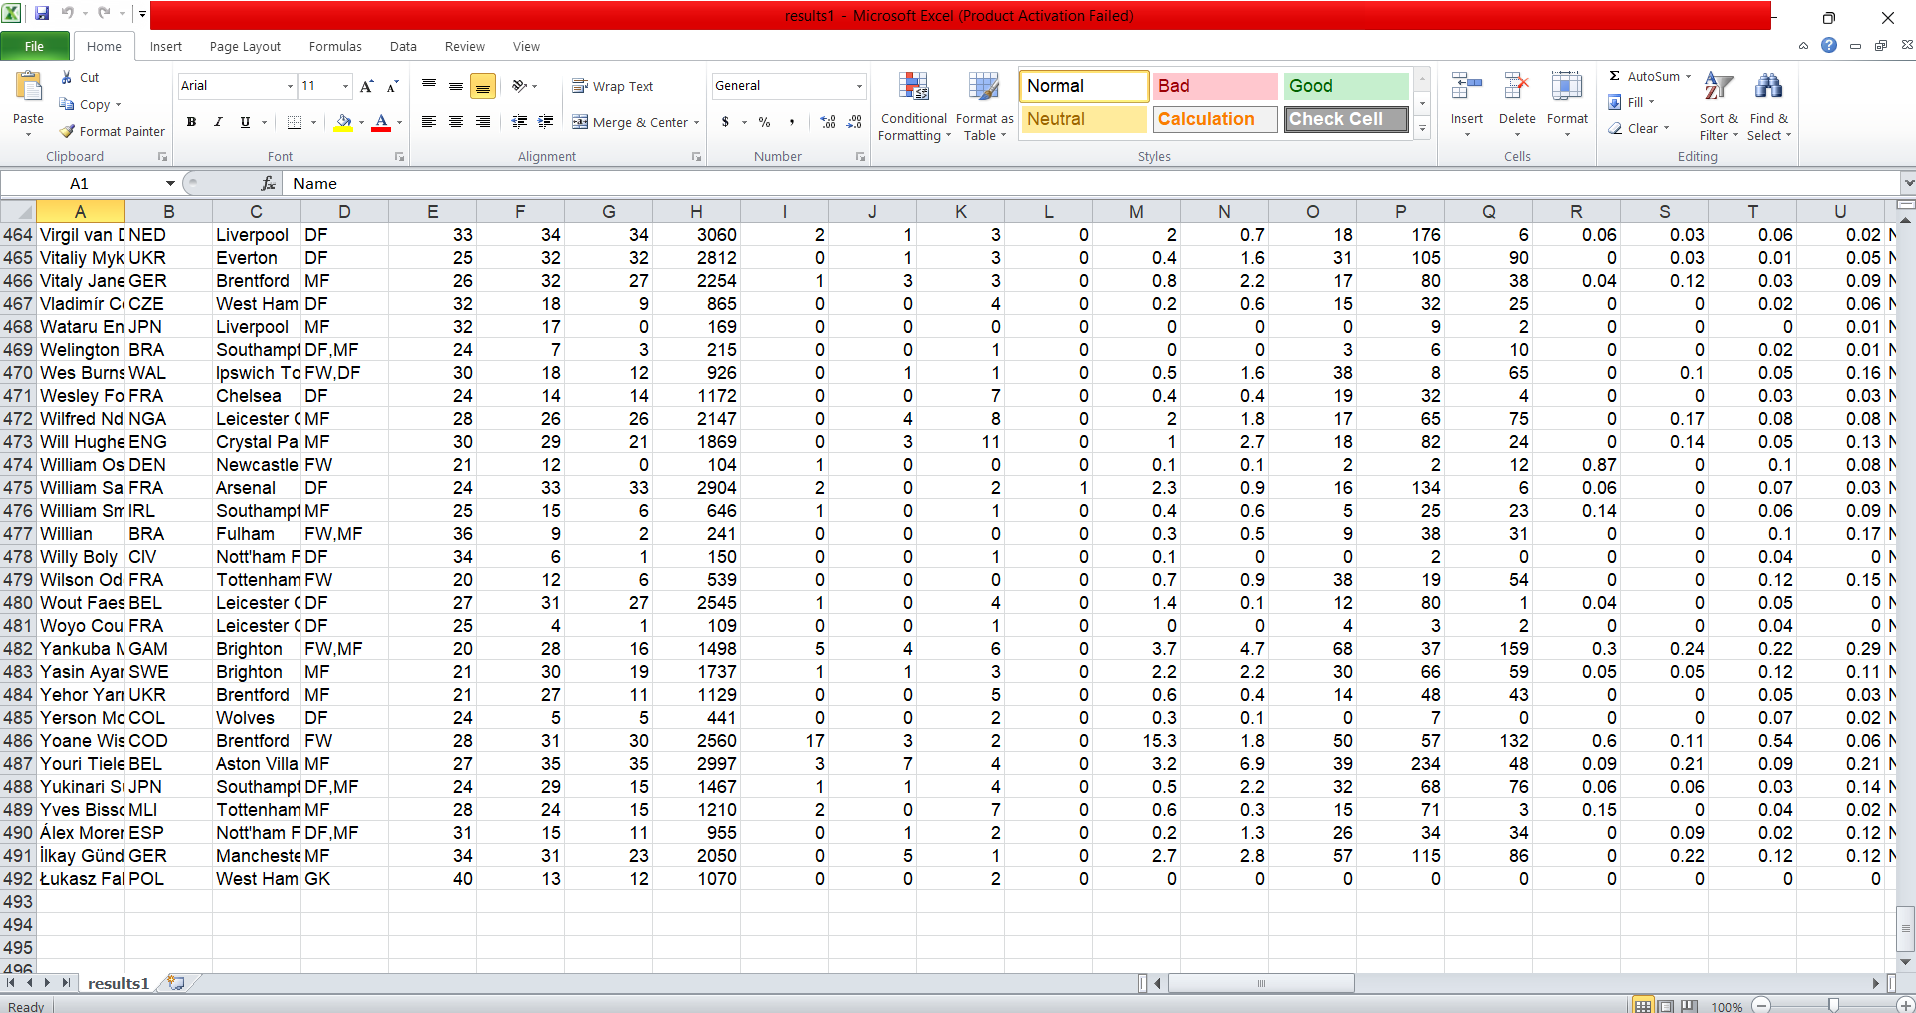
\includegraphics[width=\textwidth]{results.png}
    \caption{Image of the results.csv file}
    \label{fig:results.csv}
\end{figure}
% End of Chapter 1

% Chương 2
\chapter{Statistical Data Analysis and Visualization}

\section{Analysis of Top 3 Highest and Lowest Players per Statistical Indicator}

\subsection{Overview of Problem Requirements}
The problem requires processing a data file (\texttt{results1.csv} from the previous chapter) containing statistical information of football players.
The main objective is to identify and list the 3 players with the highest scores (Top 3) and the 3 players with the lowest scores (Bottom 3) for each statistical indicator present in the data file.
The results of this analysis are saved to a text file named \texttt{top\_3\_formatted.txt}.

\subsection{Overview of Main Code Logic \newline (\texttt{top\_3\_statistical\_analysis.py})}
The script uses the \texttt{pandas} library to read data from the CSV file.
Then, it iterates through each statistical column (excluding basic information columns such as name, nationality, team, position).
For each statistical column, the code attempts to convert the data to a numeric type, removing invalid values (\texttt{N/a} or non-convertible).
If the column can be considered numeric and contains valid data, the code will sort the data to find the top 3 highest and bottom 3 lowest values, along with the corresponding player names and teams.
Finally, the results are formatted and written to the \texttt{top\_3\_formatted.txt} file.

\subsection{Handling 'N/a'}
During data processing, \texttt{'N/a'} values are considered missing data and are converted to \texttt{NaN} via the \texttt{na\_values=['N/a']} parameter when reading the CSV file with Pandas.
Additionally, values that cannot be converted to a numeric type are also coerced to \texttt{NaN} using \texttt{pd.to\_numeric(errors='coerce')}.
Instead of replacing missing values with a specific number (like 0), entire rows containing \texttt{NaN} in the column to be evaluated are removed before performing the ranking.
This is done based on the following principles:
\begin{itemize}
    \item \textbf{Data Correctness:} \texttt{NaN} indicates that data is missing or not applicable, for example, a statistic specific to a particular position might not be relevant for a player in a different position. Replacing it with 0 would distort this characteristic.
    \item \textbf{Avoiding Misinterpretation:} Assigning a value of 0 to missing data can lead to misinterpretation – for instance, mistakenly assuming a player scored no goals, when in reality, the data was not recorded.
    \item \textbf{Ensuring Fairness in Ranking:} Considering only players with valid data helps the Top/Bottom 3 results accurately reflect actual performance, avoiding the inaccurate inclusion of individuals with missing data in comparisons.
\end{itemize}
Thus, retaining \texttt{NaN} and removing missing values from the ranking process is a reasonable method, ensuring objectivity and accuracy in player data analysis.

\subsection{Execution Steps}
\subsubsection*{Initialization and Data Preparation:}
The script imports necessary libraries (\texttt{pandas}, \texttt{os}, \texttt{numpy}, \texttt{io}).
Reads data from the \texttt{results.csv} file into a Pandas DataFrame, configured to handle \texttt{'N/a'} as \texttt{NaN}.
Identifies the list of statistical columns (\texttt{stats\_columns}) to be analyzed by excluding identifier columns ('Name', 'Team', 'Position', 'Nation').

\subsubsection*{Processing Each Column and Writing Output File:}
Opens the \texttt{top\_3\_formatted.txt} file to write the results.
The script iterates through each column \texttt{col} in \texttt{stats\_columns}:
\begin{itemize}
    \item Write Column Header: Writes the current column name to the file.
    \item Standardize & Filter Numeric Data: Uses \texttt{pd.to\_numeric(errors='coerce')} to cast the column \texttt{col} to a numeric type, converting errors to \texttt{NaN}.
    \item Creates a temporary DataFrame \texttt{df\_for\_sort} and removes rows with \texttt{NaN} values (\texttt{dropna()}) in this column.
    \item This step ensures that only valid, numeric data is used for ranking.
    \item Rank and Write Results:
    \begin{itemize}
        \item If \texttt{df\_for\_sort} contains valid numeric data: Uses \texttt{sort\_values()} to sort this DataFrame by column \texttt{col} in descending order (to find Top 3) and ascending order (to find Bottom 3), then uses \texttt{head(3)}.
        \item The results (Name, Team, Statistic) and data type information are written to the file.
    \end{itemize}
    \item Write Separator: Adds a line \texttt{===...} to separate results between columns.
\end{itemize}
Completion: After processing all columns, the \texttt{top\_3\_formatted.txt} file is saved, containing all analysis results.

\subsection{Results (\texttt{top\_3\_formatted.txt})}
The file \texttt{top\_3\_formatted.txt} contains the analysis results for each statistical indicator.
Each indicator is clearly presented with a header, followed by a list of Top 3 and Bottom 3 players.

\begin{figure}[H]
    \centering
    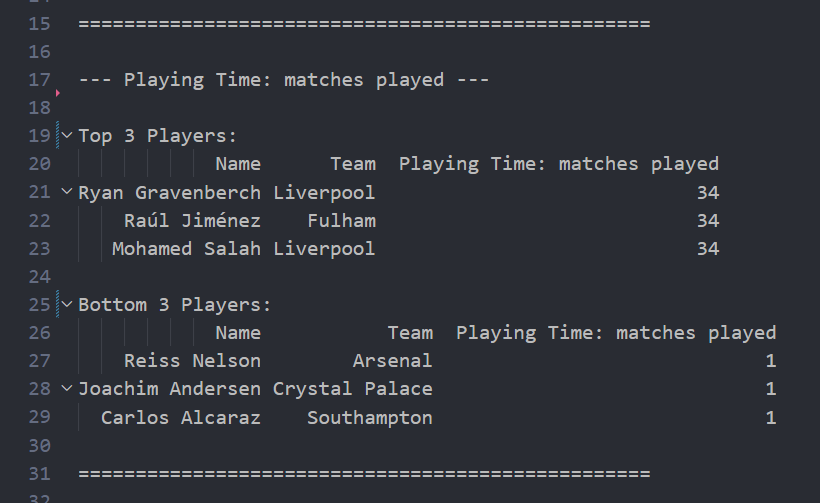
\includegraphics[width=0.8\textwidth]{top_3.png}
    \caption{Example results from the top\_3\_formatted.txt file.}
    \label{fig:top3_output}
\end{figure}

\section{Calculating Descriptive Statistics (Median, Mean, Std Dev) for Player Data}

\subsection{Introduction}
This part requires writing a Python program to perform descriptive statistical calculations on the player data collected in the previous chapter (\texttt{results1.csv}).
Specifically, the program needs to calculate:
\begin{itemize}
\renewcommand{\labelitemi}{}
    \item The median value for each statistical indicator across the entire dataset.
    \item The mean value and standard deviation for each statistical indicator, calculated for the entire dataset and separately for each team.
\end{itemize}
The results are saved to the \texttt{results2.csv} file in a specific format, where rows represent either the entirety ('all') or a specific team, and columns represent statistical calculations (Median, Mean, Std) applied to each indicator.

\subsection{Library Selection}
\begin{itemize}[leftmargin=0em]
\renewcommand{\labelitemi}{}
    \item \texttt{pandas} library: This is the primary and indispensable library for this task.
    \item \texttt{os} library: Used for flexible and OS-independent file path management. \texttt{os.path.join} and \texttt{os.path.dirname} help accurately determine the location of the input file (\texttt{results1.csv}) and output file (\texttt{results2.csv}) without hardcoding paths.
\end{itemize}

\subsection{Logic and Execution Process}
The \texttt{calculating\_statistics.py} program performs the following steps:
\begin{enumerate}[label=\textbf{Step \arabic*:}, leftmargin=*]
    \item \textbf{Prepare and Read Data:}
    Uses \texttt{os} to construct paths to the input file \texttt{results1.csv} and output file \texttt{results2.csv}.
    Reads \texttt{results.csv} into a pandas DataFrame (\texttt{df}).
    A list \texttt{na\_values\_list} containing various representations of missing values ('N/a', 'n/a', '', ...) is provided to the \texttt{na\_values} parameter of \texttt{pd.read\_csv} to ensure these values are correctly identified and converted to pandas' \texttt{NaN} (Not a Number), facilitating subsequent calculations.
    \item \textbf{Identify Statistical Columns:}
    Defines a list \texttt{exclude\_cols} containing columns that are not statistical data to be analyzed (e.g., 'Name', 'Nation', 'Team', 'Position', 'Age').
    Creates a list \texttt{stats\_columns} by filtering columns in the DataFrame, retaining only those not in \texttt{exclude\_cols}.
    \item \textbf{Calculate Overall Statistics ('all'):}
    Selects columns from \texttt{stats\_columns} in the DataFrame \texttt{df}.
    Uses the \texttt{.agg(['median', 'mean', 'std'])} method to simultaneously calculate the median, mean, and standard deviation for each column in \texttt{stats\_columns}.
    The returned result has statistical measures as rows and original columns as columns.
    Uses \texttt{.T} (transpose) to transpose the result, making the original statistic names (\texttt{stats\_columns}) the row index, and 'median', 'mean', 'std' the column names, saving it into \texttt{overall\_stats}.
    This facilitates easier access in the next step.
    \item \textbf{Calculate Grouped Statistics ('Team'):}
    Uses \texttt{df.groupby('Team')} to group the DataFrame by values in the 'Team' column.
    On this GroupBy object, selects the \texttt{stats\_columns}.
    Applies \texttt{.agg(['median', 'mean', 'std'])} to calculate statistics for each team.
    The result (\texttt{team\_stats}) will have a MultiIndex structure for both rows (Team) and columns (Statistic, Metric).
    \item \textbf{Restructure Data for Output:}
    \begin{itemize}[leftmargin=0em]
        \item Create 'all' row: Initializes an empty DataFrame \texttt{all\_row} with 'all' as its index. Iterates through each statistical column (\texttt{col} in \texttt{stats\_columns}), creating new columns in \texttt{all\_row} named in the format \texttt{f'Median of \{col\}'}, \texttt{f'Mean of \{col\}'}, \texttt{f'Std of \{col\}'} and assigns corresponding values from \texttt{overall\_stats} calculated in Step 3.
        \item Create 'Team' rows: Initializes a DataFrame \texttt{team\_results} with team names as its index (obtained from \texttt{team\_stats.index}). Iterates through each statistical column (\texttt{col} in \texttt{stats\_columns}), creating new columns in \texttt{team\_results} with similarly formatted names as above. Values are retrieved from \texttt{team\_stats} by accessing through the multi-level index, e.g., \texttt{team\_stats[(col, 'median')]} to get the median column for statistic \texttt{col}.
        \item Combine Results: Uses \texttt{pd.concat([all\_row, team\_results])} to concatenate the DataFrame containing the 'all' row and the DataFrame containing individual team rows vertically, forming the final DataFrame \texttt{final\_results} with the required structure.
    \end{itemize}
    \item \textbf{Save Results:}
    Exports the \texttt{final\_results} DataFrame to the \texttt{results2.csv} file using the \texttt{.to\_csv()} method.
    The \texttt{index=True} parameter is used (by default) to save the DataFrame's index ('all' or team name) into the first column of the CSV file.
\end{enumerate}

\subsection{Results}
The program ran successfully and generated the \texttt{results2.csv} file.
The \texttt{results2.csv} file contains the aggregated statistical results in the required format:
\begin{itemize}
    \item Rows: The first row has an index 'all', representing statistics for all players. Subsequent rows have indices corresponding to team names, representing statistics calculated separately for players of that team.
    \item Columns: Columns are named following the pattern "Metric of Statistic", e.g., "Median of Performance: goals", "Mean of Performance: goals", "Std of Performance: goals", "Median of Performance: assists", etc., including all indicators in \texttt{stats\_columns}.
    \item Values: Cells contain the corresponding calculated median, mean, or standard deviation values. NaN values (if any, e.g., standard deviation for a group with only 1 player) will be represented as empty cells in the CSV file.
\end{itemize}

\begin{figure}[H]
    \centering
    % Thay 'image_results2_csv_example.png' bằng tên file ảnh thực tế của bạn
    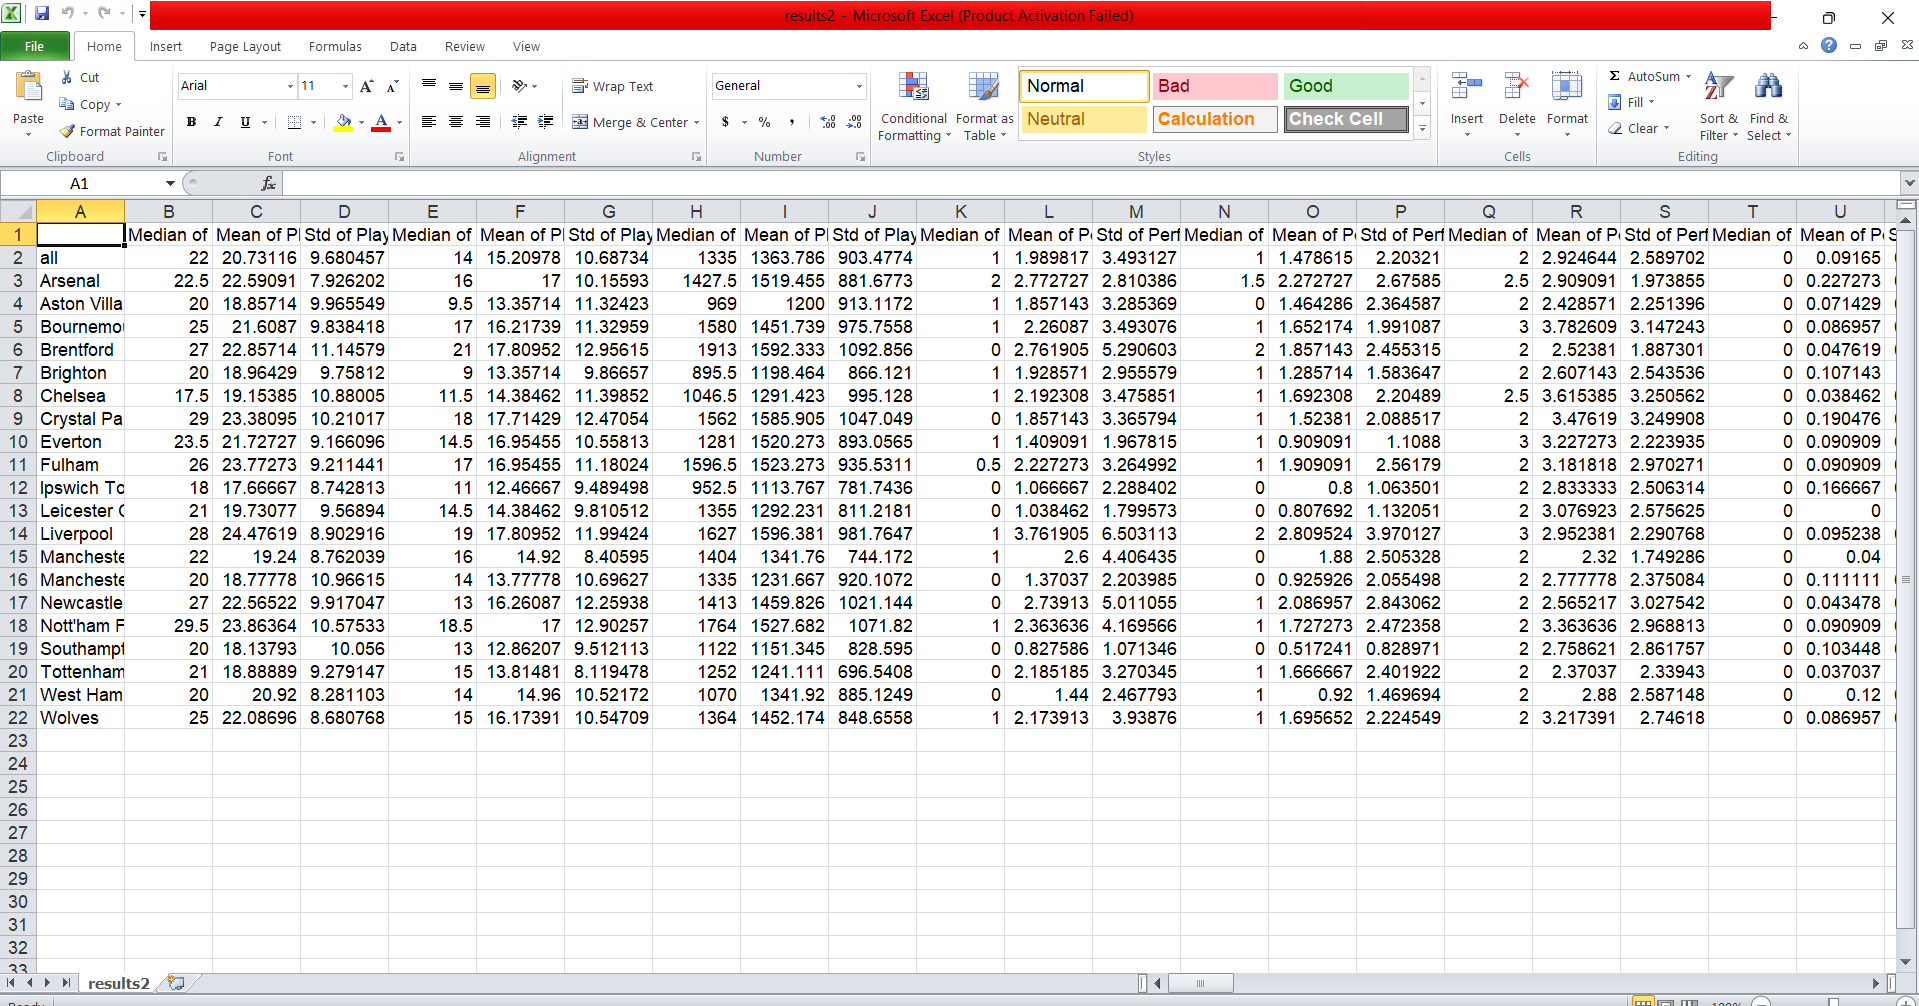
\includegraphics[width=\textwidth]{results2.png}
    \caption{Example data from the results2.csv file.}
    \label{fig:results2_csv}
\end{figure}

\section{Visualizing Player Statistical Distribution using Histograms}

\subsection{Objectives}
The main objective of the \texttt{plot\_stat\_histograms.py} script is to visualize and analyze the distribution of a set of important statistical indicators for football players.
Specifically, the script aims to:
\begin{itemize}
    \item Generate histograms for each selected statistical indicator (\texttt{stats\_to\_plot}) to show its distribution across the \textit{entire league} (all players).
    \item Generate separate histograms for each \textit{football team}, showing the distribution of each statistical indicator within that team.
    \item Save these charts as image files (PNG) for easy review, sharing, and later analysis.
    \item Provide a visual understanding of the distribution shape (e.g., symmetric, left-skewed, right-skewed), central tendency, and dispersion of statistical indicators, both at the league level and team level.
\end{itemize}
The specific statistical indicators analyzed in this script include: \texttt{'Performance: goals'}, \texttt{'Performance: assists'}, \texttt{'Standard: shoots on target percentage (SoT\%)'}, \texttt{'Blocks: Int'}, \texttt{'Performance: Recov'}, \texttt{'Challenges: Att'}.

\subsection{Library Selection}
The script uses several common Python libraries for data processing and visualization:
\begin{itemize}
    \item \texttt{pandas}: The core library for reading data from CSV files (\texttt{results1.csv}), storing data in DataFrames, and performing necessary data manipulation, filtering, and selection for plotting. It also handles missing values (NaN).
    \item \texttt{matplotlib.pyplot}: The foundational library for creating charts in Python. It is used to create figures, axes, set titles, labels, and manage chart layouts, especially when plotting multiple subplots for teams.
    \item \texttt{seaborn}: A library built on \texttt{matplotlib}, providing a higher-level interface for drawing attractive and informative statistical graphics. Specifically, \texttt{seaborn.histplot} is used to draw histograms, including a kernel density estimate (KDE) line that helps smooth and better visualize the distribution shape. \texttt{seaborn.set\_theme} is used to set the overall aesthetic style for the charts.
    \item \texttt{numpy}: A scientific computing library, used in the \texttt{calculate\_fd\_bins} function to perform necessary calculations (like cube root \texttt{np.cbrt}, base-2 logarithm \texttt{np.log2}) for determining the optimal number of bins according to the Freedman-Diaconis and Sturges rules.
    \item \texttt{os}: A library providing functions for interacting with the operating system, mainly used for managing file paths (getting current directory path, joining paths), creating storage directories (\texttt{stat\_histograms}), and ensuring valid paths.
    \item \texttt{math}: A basic math library, used for functions like \texttt{math.ceil} to round up when calculating the number of rows/columns for subplots and the number of bins.
\end{itemize}

\subsection{Execution Steps}
The script performs the following main steps:
\subsubsection*{Configuration Setup}
Defines constants such as the output directory (\texttt{OUTPUT\_DIR}), the column name containing team information (\texttt{TEAM\_COL}), the maximum number of teams per plot (\texttt{TEAMS\_PER\_PLOT}), plot style (\texttt{PLOT\_STYLE}), and the maximum bin limit (\texttt{MAX\_FD\_BINS}).

\subsubsection*{Defining Helper Functions}
\begin{itemize}
    \item \texttt{ensure\_dir}: Ensures the output directory exists.
    \item \texttt{sanitize\_filename}: Cleans the statistical indicator name to create a valid filename.
    \item \texttt{calculate\_fd\_bins}: Calculates the optimal number of bins for a histogram based on the Freedman-Diaconis rule (preferred) or Sturges' rule (fallback), helping the chart better reflect the actual data structure and avoid arbitrary bin selection. There is a maximum bin limit to prevent excessive detail.
\end{itemize}

\subsubsection*{Defining Plotting Functions}
\begin{itemize}
    \item \texttt{plot\_overall\_hist}:
    \begin{itemize}
        \item Takes a DataFrame, statistical indicator name, and output directory as input.
        \item Filters data for the statistical indicator, converts to numeric type, and removes missing values (\texttt{NaN}).
        \item Calculates the optimal number of bins using \texttt{calculate\_fd\_bins}.
        \item Uses \texttt{seaborn.histplot} to draw the overall distribution histogram, with KDE enabled.
        \item Sets title, axis labels, and saves the chart to a PNG file with a standardized name.
    \end{itemize}
    \item \texttt{plot\_team\_hist}:
    \begin{itemize}
        \item Takes a DataFrame, indicator name, output directory, team column name, and number of teams per figure as input.
        \item Gets a list of unique teams and divides them into smaller groups \sloppypar
 (according to \texttt{TEAMS\_PER\_PLOT}).
        \item Iterates through each group of teams:
        \begin{itemize}
            \item Creates a new figure with subplots (a grid of smaller charts).
            \item Filters data to include only teams in the current group.
            \item Calculates the optimal number of bins \textit{based on the data range of teams in this group}. This helps histograms within the same figure share a common way of dividing value ranges.
            \item Determines common x-axis limits (\texttt{x\_min}, \texttt{x\_max}) for all subplots in the current figure for easier comparison.
            \item Draws a histogram for each team on a separate subplot using \texttt{seaborn.histplot}, using the calculated number of bins and bin range (\texttt{binrange}).
            \item Sets the subplot title as the team name, hides axis labels to avoid clutter, and applies uniform x-axis limits.
            \item Hides any unused subplots.
            \item Sets the main title for the figure (including indicator name and team group).
            \item Saves the figure containing histograms for the group of teams to a PNG file.
        \end{itemize}
    \end{itemize}
\end{itemize}

\subsubsection*{Main Execution Block (\texttt{if \_\_name\_\_ == '\_\_main\_\_':})}
\begin{itemize}
    \item Sets the theme for \texttt{seaborn}.
    \item Defines the list of indicators to plot (\texttt{stats\_to\_plot}).
    \item Determines the path and reads the \texttt{results.csv} file into a DataFrame.
    \item Ensures the output directory exists.
    \item Iterates through each indicator in \texttt{stats\_to\_plot}:
    \begin{itemize}
        \item Calls \texttt{plot\_overall\_hist} to plot the overall histogram.
        \item Calls \texttt{plot\_team\_hist} to plot histograms for each team (grouped).
    \end{itemize}
\end{itemize}

\subsection{Visual Results}
The output of the script is a set of PNG image files saved in the \texttt{stat\_histograms} directory.
Specifically:
\begin{itemize}
    \item For each statistical indicator in \texttt{stats\_to\_plot}, there will be \textit{one file} containing a histogram showing the overall distribution of that indicator across the entire league \sloppypar
    (e.g., \texttt{hist\_overall\_Standard\_shoots\_on\_target\_percentage\_SoT.png}).
\end{itemize}

\begin{figure}[H]
    \centering
    % Thay 'image_hist_overall_sot.png' bằng tên file ảnh thực tế của bạn
    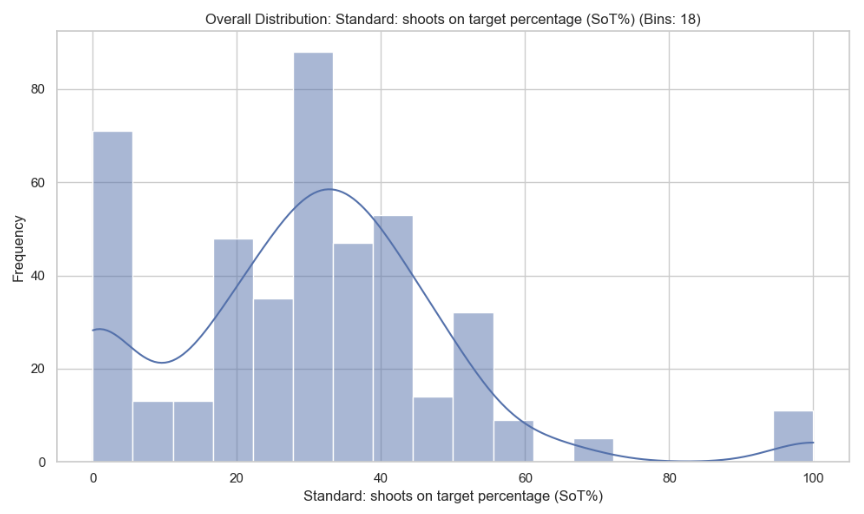
\includegraphics[width=0.8\textwidth]{overall.png}
    \caption{Example of an overall histogram (Source: Excerpt from original document).}
    \label{fig:hist_overall_sot}
\end{figure}

\begin{itemize}
    \item For each statistical indicator, there will be \textit{one or more files} of histograms showing its distribution per team. Teams are grouped (default 20 teams/figure) to avoid creating too many files or overly large images \sloppypar
    (e.g., \texttt{hist\_teams\_Standard\_shoots\_on\_target\_percentage\_SoT\_group\_1.png},...).
\end{itemize}

\begin{figure}[H]
    \centering
    % Thay 'image_hist_teams_sot_group1.png' bằng tên file ảnh thực tế của bạn
    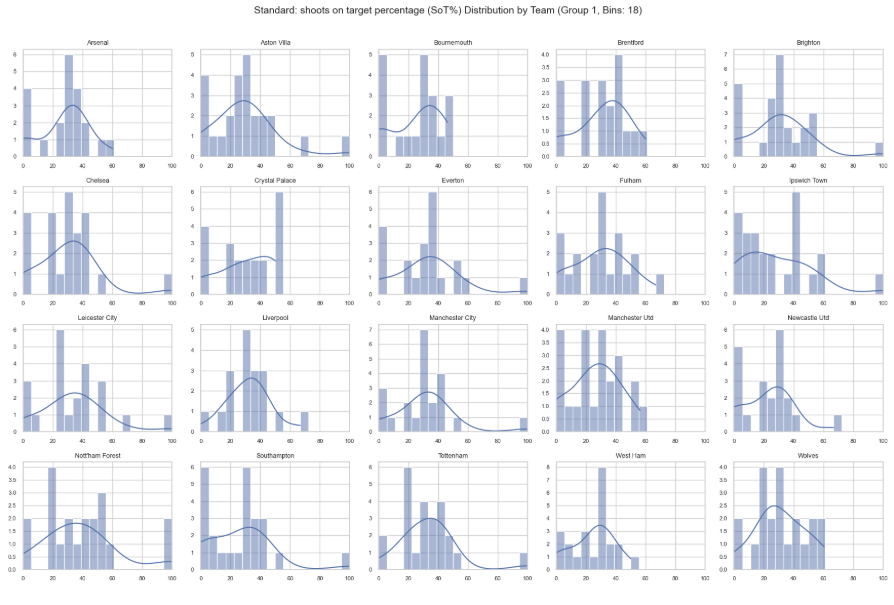
\includegraphics[width=\textwidth]{by_team.png}
    \caption{Example of histograms by team group (Source: Excerpt from original document).}
    \label{fig:hist_teams_sot_group1}
\end{figure}

Each of these files contains a grid of small charts, with each small chart corresponding to a team.
These charts allow viewers to visually observe the distribution shape (symmetric, skewed, multimodal), value range, and frequency of different values for each indicator, both overall and within each team.

\subsection{Limitations}
In the process of analyzing player statistical data, histograms are used to visualize the distribution of each indicator (e.g., number of goals, minutes played, assists, etc.).
This is an effective tool for quickly observing common trends, detecting outliers, and comparing differences between players or teams.
However, the use of histograms also has some limitations that need to be noted to avoid drawing inaccurate or biased conclusions:
\begin{itemize}
    \item \textbf{Dependency on Data Quality:} The visual results are entirely dependent on the completeness and accuracy of the data in the \texttt{results.csv} file. Missing values (\texttt{NaN}) were removed during processing to ensure the accuracy of the charts. However, if the proportion of missing data is large or not randomly distributed, this can distort the distribution shape and lead to biased judgments about overall trends.
    \item \textbf{Sensitivity to the Number of Bins:} Although the number of bins is determined based on the Freedman-Diaconis rule to optimize the level of detail in the chart, the histogram's shape can still change if the number of bins is altered. Furthermore, setting a maximum limit for the number of bins (via the \texttt{MAX\_FD\_BINS} variable) is subjective and can affect the chart's resolution, especially in distributions with many dispersed values.
\end{itemize}

\section{Performance Analysis of Premier League Teams 2024–2025}

\subsection{Introduction}
To evaluate the performance of teams in the 2024–2025 season, the analysis process is designed with two main objectives: identifying the leading team for each statistical indicator and finding the team with the best overall performance.
Data processing is carried out using two main files:
\begin{itemize}
    \item \texttt{highest\_stats\_team.py}: The Python source code file that handles the entire analysis process, from reading data, classifying indicators (good, bad, ignore), determining the leading team for each criterion, to aggregating results to identify the best-performing team of the season.
    \item \texttt{config.json}: A configuration file that allows flexible customization of parameters such as data paths, handling of missing values, and the indicator classification system. Separating the configuration helps adjust analysis criteria without modifying the source code.
\end{itemize}
This approach optimizes reusability, maintainability, and scalability for different seasons or datasets.

\subsection{Main Idea}
\begin{itemize}[leftmargin=0em]
\renewcommand{\labelitemi}{}
    \item \textbf{Identify the team with the highest score for each indicator:} The script classifies indicators into three groups (good, bad, ignore) based on the configuration file (\texttt{config.json}). For each indicator, the code converts the data to a numeric type, then finds the optimal value (highest for good indicators, lowest for bad indicators) and identifies which team achieved that value. For example, the team with the most goals, the team with the highest pass completion rate, or the team with the fewest red cards.
    \item \textbf{Identify the team with the best overall performance:} The code counts the number of times each team leads in different indicators, separately for good and bad indicators. Then, it calculates a combined total score for each team by summing the number of times they led in both types of indicators. The team with the highest total number of leading instances is considered the team with the best overall performance in the season.
\end{itemize}

\subsection{Execution Process}
The analysis process is controlled by the \texttt{highest\_stats\_team.py} script, with the following main steps:
\subsubsection*{Initialization & Load Configuration}
Loads configuration from \texttt{config.json} using the \texttt{load\_config} function. This function reads the JSON file and creates sets of keywords \texttt{ignore\_stats\_set}, \texttt{bad\_stats\_set}, \texttt{good\_stats\_set} for classifying indicators.

\subsubsection*{Define Path & Read CSV Data}
Constructs the absolute path to the \texttt{results2.csv} file (located in \texttt{../calculating\_statistics/}).
Reads data from CSV into a DataFrame \texttt{dataframe} using \texttt{pandas}, utilizing \texttt{na\_values} from the config.

\subsubsection*{Preprocess DataFrame}
Identifies the team name column (defaults to the first column).
Standardizes the team name column: converts to lowercase, removes rows where the team name is "all".

\subsubsection*{Determine Leading Team for Each Valid Statistic \sloppypar (Function \texttt{analyze\_performance\_by\_stat\_type})}
\begin{enumerate}[label*=\textbf{Step \arabic*:}, leftmargin=*]
    \item Identify and Filter Indicators for Analysis:
    \begin{itemize}[leftmargin=0em]
        \item Create a list of columns prefixed with "Mean of " (excluding the team column).
        \item For each potential column:
        \begin{itemize}
            \item Extract the actual indicator name (remove "Mean of ").
            \item Classify the indicator (using \texttt{classify\_stat}) as 'ignore', 'bad', 'good', or 'uncategorized' based on the loaded keyword sets.
            \item If not 'ignore', convert the column to numeric. Only retain indicators with at least one valid numeric value.
        \end{itemize}
    \end{itemize}
    \item Analyze Each Filtered Indicator:
    \begin{itemize}[leftmargin=0em]
        \item For each indicator selected for analysis:
        \begin{itemize}
            \item Convert the indicator column to numeric and remove invalid values (\texttt{NaN}).
            \item Find the best value:
            \begin{itemize}
                \item If type is 'good' or 'uncategorized': find the \textit{maximum} value.
                \item If type is 'bad': find the \textit{minimum} value.
            \end{itemize}
            \item If the best value is not found (e.g., empty column), log an error.
            \item Otherwise:
            \begin{itemize}
                \item Identify the team(s) achieving this best value.
                \item Save the name(s) of the leading team(s), the best value (in its original format for display), and the indicator type into a results dictionary.
            \end{itemize}
        \end{itemize}
    \end{itemize}
    \item Return: Dictionary containing analysis results for each indicator.
\end{enumerate}

\subsubsection*{Display Detailed Analysis Results}
Sorts results by indicator name.
Iterates through each analyzed indicator, formats the value (using \texttt{format\_value} to handle integers, floats, "N/A"), and prints: indicator name, type (GOOD, BAD), leading team, and achieved value.

\subsubsection*{Calculate and Display Consolidated Ranking Table}
\begin{enumerate}[label*=\textbf{Step \arabic*:}, leftmargin=*]
    \item Count Leading Instances:
    \begin{itemize}[leftmargin=0em]
        \item For each indicator with valid results in \texttt{analysis\_results}:
        \begin{itemize}
            \item If a team leads a 'good' indicator, increment its score in \texttt{good\_lead\_counts}.
            \item If a team leads a 'bad' indicator, increment its score in \texttt{bad\_lead\_counts}.
        \end{itemize}
    \end{itemize}
    \item Create Consolidated Score:
    \begin{itemize}[leftmargin=0em]
        \item Get a list of all unique teams from the DataFrame.
        \item Initialize a score of 0 for all teams.
        \item Sum the total 'good' and 'bad' leading instances to get a consolidated score for each team.
    \end{itemize}
    \item Sort and Display:
    \begin{itemize}[leftmargin=0em]
        \item Sort teams: descending by consolidated score, then ascending by team name (if scores are tied).
        \item Print the ranking table with rank, team name, and total leading instances.
    \end{itemize}
\end{enumerate}

\subsection{Results}
When the \texttt{highest\_stats\_team.py} script is executed successfully, it will produce two main blocks of information printed to the console (command line interface).
These results provide a detailed view of each team's performance for every analyzed statistical indicator, and a consolidated ranking table of teams based on the number of times they led those indicators.

\begin{figure}[H]
    \centering
    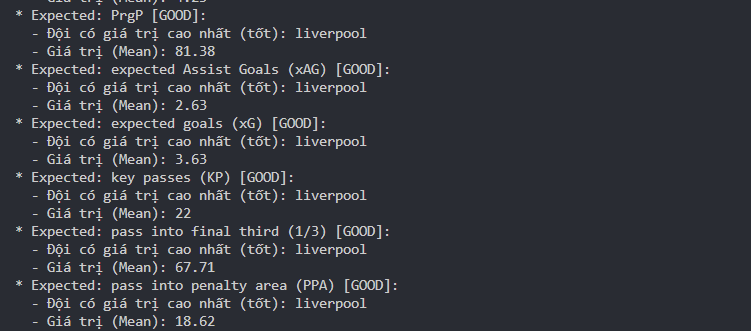
\includegraphics[width=0.8\textwidth]{output_2.4.1.png}
    \caption{Example of detailed analysis results by indicator.}
    \label{fig:analysis_output1}
\end{figure}

\begin{figure}[H]
    \centering
    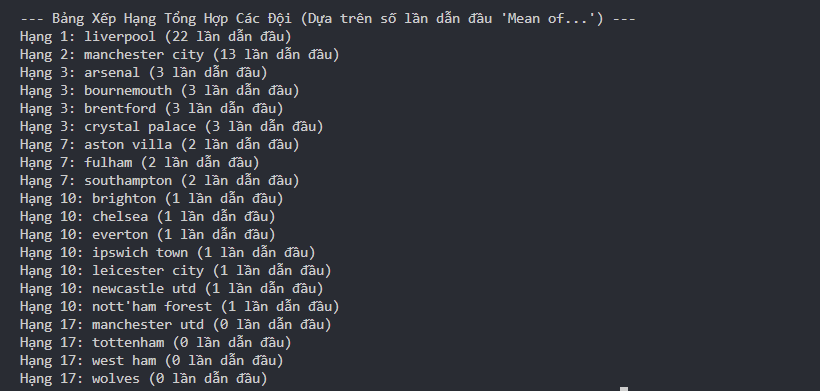
\includegraphics[width=0.8\textwidth]{output_2.4.2.png}
    \caption{Example of consolidated team ranking table.}
    \label{fig:overall_ranking}
\end{figure}

The statistical data indicates that Liverpool is an outstanding and comprehensive team, not only excelling in a few aspects but also maintaining impressive form across most crucial indicators of modern football.
They possess explosive attacking power, superior ball control, and a solid defensive system – all contributing to a smooth and effective playing machine.
In reality, they convincingly won the Premier League title for the 2024–2025 season \textit{with 4 matches to spare}, accumulating \textit{82 points} – a safe distance ahead of the runner-up, Arsenal.
This is clear evidence that when a football team operates correctly in terms of both expertise and strategy, its dominance will be clearly reflected in the statistical numbers and on-field results.
% End of Chapter 2

% Chương 3
\chapter{Player Clustering and Dimensionality Reduction with PCA}

\section{Football Player Clustering using K-means Algorithm}

\subsection{Introduction}
Player data analysis plays a crucial role in modern sports, helping coaches, analysts, and managers make informed decisions.
One of the common techniques used is the K-means clustering algorithm, which aims to divide a set of players into distinct groups (clusters) based on the similarity of their statistical indicators.
This section will present how the K-means algorithm is applied, particularly focusing on determining the optimal number of clusters and commenting on the results obtained from running the source code file \texttt{player\_clustering\_kmeans.py}.

\subsection{Selecting the Range of k for Experimentation}
Selecting the range of $k$ for experimentation in the player clustering problem (500 players, 78 indicators) needs to be based on theoretical factors, data characteristics, and practical context in football.

\subsubsection*{Reasons for Choosing kmin = 3}
\begin{itemize}
    \item \textbf{Minimum requirement for meaningful clustering:}
    \begin{itemize}
        \item k=1: does not create clusters (all data belongs to the same group), no analytical value.
        \item k=2: only divides data into two groups, often too simplistic for data with around 78 indicators (only providing a crude distinction like "attack" and "defense").
        \item k=3: a reasonable starting point to reflect basic roles in football, e.g., goalkeeper, defender, attacker.
    \end{itemize}
    \item \textbf{Suitability for sample size:}
    \begin{itemize}
        \item With 500 players, k=3 creates clusters averaging $500/3 \approx 167$ players/cluster, large enough to be statistically significant.
    \end{itemize}
\end{itemize}
\textbf{Conclusion:} kmin=3 is a reasonable starting point.

\subsubsection*{Reasons for Choosing kmax = 15}
\begin{itemize}
    \item \textbf{Based on sample size (around 500 players):}
    \begin{itemize}
        \item Each cluster should have at least 20–50 samples to ensure statistical significance:
        \begin{itemize}
            \item If each cluster has a minimum of 20 players: $k = 500/20 = 25$
            \item If each cluster has a minimum of 50 players: $k = 500/50 = 10$.
        \end{itemize}
        \item To ensure clusters are not too small, kmax should be in the range of 10–25. However, context needs further consideration.
    \end{itemize}
    \item \textbf{Football context:}
    \begin{itemize}
        \item The number of roles/playing styles in football rarely exceeds 15–20 (e.g., goalkeeper, center-back, full-back, defensive midfielder, attacking midfielder, winger, center-forward, deep-lying forward, etc.).
        \item k=15 is sufficient to cover detailed roles without exceeding practical limits.
    \end{itemize}
    \item \textbf{Practical experience:}
    \begin{itemize}
        \item In similar clustering problems, kmax=15 is often sufficient to cover elbow points (typically occurring in the range k=4 to k=10), avoiding wasted computational resources.
    \end{itemize}
\end{itemize}
\textbf{Conclusion:} kmax=15 is a reasonable threshold.
The range of k from 3 to 15 is reasonable: kmin=3 creates basic clusters (167 players/cluster), kmax=15 covers detailed roles (33 players/cluster), suitable for the data, football context, and elbow points typically found between k=4 and k=10.

\subsection{Determining the Optimal Number of Clusters (K) and Execution Process}
\textbf{Main Idea:} To determine the optimal number of clusters (K) for grouping players, I applied the Elbow method.
This process begins by experimenting with the K-Means algorithm using a range of potential K values, specifically from 3 to 15 clusters.
For each K value, the WCSS (Within-Cluster Sum of Squares - the sum of squared distances from each data point to its cluster center) is calculated.
WCSS is a measure of cluster cohesion; a lower WCSS value indicates that data points within the same cluster are closer to each other.
Subsequently, these WCSS values are visualized on a line graph, with the number of clusters (K) on the x-axis and the corresponding WCSS on the y-axis.
The "elbow point" on the graph, where increasing the number of clusters K no longer leads to a significant decrease in WCSS, is identified as the optimal K value.
Based on the analysis of the Elbow plot, a suitable K value was chosen.
Finally, the K-Means algorithm is re-executed with this optimal K number of clusters to divide the players into corresponding groups, whereby each player is assigned to a cluster based on statistical similarity.

\subsubsection*{Configuration and Initialization}
\begin{itemize}
    \item \textbf{Import libraries:} Loads necessary libraries such as \texttt{pandas}, \texttt{numpy}, \texttt{os}, \texttt{sklearn.cluster.KMeans} (for the K-Means algorithm), \texttt{sklearn.preprocessing.StandardScaler} (for data standardization), \texttt{sklearn.impute.SimpleImputer} (for handling missing values), \texttt{matplotlib.pyplot}, and \texttt{seaborn} (for plotting).
    \item \textbf{Define configuration constants:}
    \begin{itemize}
        \item \texttt{PLAYER\_COL}: Name of the column containing player names (default is 'Name').
        \item \texttt{CSV\_RELATIVE\_PATH}: Relative path to the CSV file containing player data (default is \texttt{../problem\_1/results1.csv}).
        \item \texttt{script\_dir}: Gets the current directory path of the script.
        \item \texttt{output\_folder\_name}: Name of the folder to save analysis results (default is \texttt{kmeans\_analysis\_results}).
        \item \texttt{OUTPUT\_DIR}: Creates an absolute path to the directory for saving results.
    \end{itemize}
    \item \textbf{Define helper function \texttt{ensure\_dir(path: str)}:} This function ensures that a directory exists at the provided path; if not, it creates the directory.
\end{itemize}

\subsubsection*{Main function \texttt{cluster\_players\_kmeans(csv\_path: str, player\_col: str, max\_k: int = 10)}}
\begin{itemize}
    \item \textbf{Load Data:}
    \begin{itemize}
        \item Determine the absolute path to the CSV file.
        \item Read data from the CSV file into a \texttt{pandas} DataFrame.
    \end{itemize}
    \item \textbf{Prepare Data:}
    \begin{itemize}
        \item Select numeric columns: Identify and select all columns in the DataFrame with numeric data types to be used as features for clustering (also excluding the ‘Age’ column to make clusters more clearly reflect similarities in skills, playing style, or tactical roles, rather than being influenced by the player's career stage).
        \item Handle missing values (NaN): Use \texttt{SimpleImputer} to replace any missing values in the selected numeric columns with the mean of the respective column.
        \item Standardize Data: Use \texttt{StandardScaler} to standardize the numeric features. This ensures that all features are on the same scale, which is crucial for distance-based algorithms like K-Means.
    \end{itemize}
    \item \textbf{Determine the optimal number of clusters (K) using the Elbow method:}
    \begin{itemize}
        \item Initialize a list \texttt{wcss} (Within-Cluster Sum of Squares).
        \item Iterate over a range of possible K values (from 3 to 15).
        \item For each K value:
        \begin{itemize}
            \item Create a K-Means model (\texttt{KMeans}) with K clusters, initialization method \texttt{'k-means++'}, \texttt{n\_init='auto'} (to automatically choose the number of runs with different centroid seeds), and \texttt{random\_state=42} (to ensure reproducible results).
            \item Train the K-Means model on the standardized data.
            \item Get the \texttt{inertia\_} (WCSS) value of the model and add it to the \texttt{wcss} list.
        \end{itemize}
        \item Plot the Elbow graph:
        \begin{itemize}
            \item Call the \texttt{ensure\_dir} function to create the output directory if it doesn't exist.
            \item Create a line plot (\texttt{plot}) with the number of clusters (K) on the x-axis and WCSS on the y-axis.
            \item Set the title, axis labels, and display a grid for the plot.
            \item Save the Elbow plot as a PNG file in the \texttt{OUTPUT\_DIR} directory.
        \end{itemize}
        \item Print a message guiding the user to view the plot and select the optimal K value (the "elbow" point on the plot, where WCSS begins to decrease more slowly).
    \end{itemize}
    \item \textbf{Get optimal K input from the user:}
    \begin{itemize}
        \item Prompt the user to enter the optimal number of clusters K based on the Elbow plot.
        \item The loop continues until the user inputs a valid integer within the allowed range.
    \end{itemize}
    \item \textbf{Apply K-means with optimal K:}
    \begin{itemize}
        \item After the user selects K, create a final K-Means model with the chosen \texttt{optimal\_k} number of clusters.
        \item Train this final K-Means model on the standardized data.
        \item Get the cluster labels assigned to each data point (each player).
    \end{itemize}
    \item \textbf{Add cluster labels to the original DataFrame:}
    \begin{itemize}
        \item Create a copy of the original DataFrame.
        \item Add a new column named \texttt{'Cluster'} to this copy, containing the assigned cluster labels.
    \end{itemize}
    \item \textbf{Analyze and Save Results:}
    \begin{itemize}
        \item Analyze cluster centroids:
        \begin{itemize}
            \item Calculate the centroid coordinates of each cluster on the standardized scale (\texttt{final\_kmeans.cluster\_centers\_}).
            \item Transform these centroid coordinates back to the original scale using \texttt{scaler.inverse\_transform()}.
            \item Create a new DataFrame (\texttt{centroid\_df}) containing the mean values of numeric features for each cluster (on the original scale).
            \item Print this centroid DataFrame (rounded to 2 decimal places).
            \item Save the centroid DataFrame to a CSV file in the \texttt{OUTPUT\_DIR} directory.
        \end{itemize}
        \item Count players in each cluster: Print the number of players belonging to each cluster.
        \item Sort and Save Clustered DataFrame:
        \begin{itemize}
            \item Sort the DataFrame with assigned cluster labels by the \texttt{'Cluster'} column.
            \item Save this sorted DataFrame to another CSV file in the \texttt{OUTPUT\_DIR} directory.
        \end{itemize}
    \end{itemize}
    \item \textbf{Return} the clustered DataFrame, the \texttt{scaler} object, the standardized features DataFrame, and the list of numeric columns.
\end{itemize}

\subsubsection*{Main execution block (\texttt{if \_\_name\_\_ == '\_\_main\_\_':})}
\begin{itemize}
    \item \textbf{Call clustering function:} Call the \texttt{cluster\_players\_kmeans} function with configured parameters (\texttt{CSV\_RELATIVE\_PATH}, \texttt{PLAYER\_COL}).
    \item \textbf{Store returned results} (clustered DataFrame, scaler, etc.).
    \item \textbf{Display example players from each cluster (if clustering is successful):}
    \begin{itemize}
        \item Check if \texttt{clustered\_data} exists.
        \item If it exists and the \texttt{numeric\_cols\_list} is not empty:
        \begin{itemize}
            \item Iterate through each unique cluster ID (sorted).
            \item Print the header for that cluster.
            \item Get the first 5 players (\texttt{head(5)}) from the current cluster.
            \item Select columns to display: player name (\texttt{PLAYER\_COL}), at most the first 5 numeric features, and the \texttt{'Cluster'} column.
            \item Print the information for these sample players.
        \end{itemize}
    \end{itemize}
\end{itemize}

\subsection{K-means Clustering Results}


\begin{figure}[H]
    \centering
    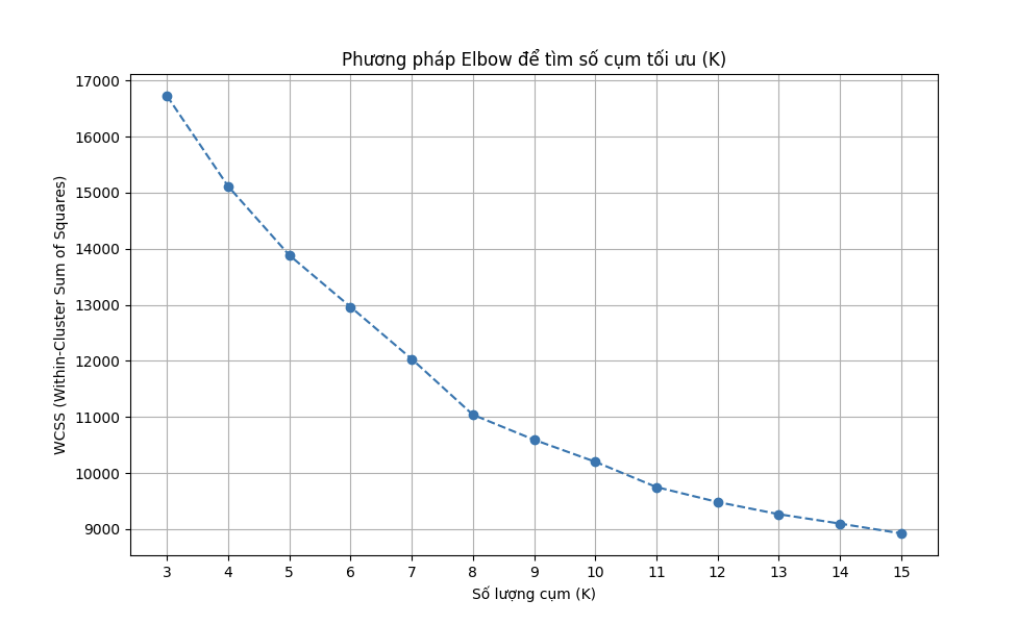
\includegraphics[width=\textwidth]{Elbow.png}
    \caption{Elbow method for finding the optimal number of clusters (K).}
    \label{fig:elbow_method}
\end{figure}

The Elbow plot shows a sharp decrease in WCSS from k = 3 (17000) to k = 6 (12000), then a slower decrease from k = 6 to k = 15 (down to 9000), marking k = 6 as the "elbow" point.
Choosing k = 6 is reasonable as it balances clustering quality (WCSS has significantly decreased) and model complexity, avoiding the creation of unnecessary additional clusters when WCSS subsequently decreases insignificantly.
The number of players in each cluster will be printed to the screen.

\begin{figure}[H]
    \centering
    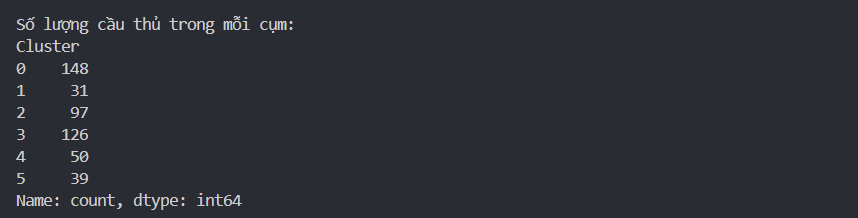
\includegraphics[width=\textwidth]{cluster.png}
    \caption{Number of players in each cluster.}
    \label{fig:players_per_cluster}
\end{figure}


The mean values of each indicator within each cluster are saved to the \texttt{cluster\_centroids.csv} file, while the detailed clustering results for each player are saved to the \texttt{player\_clusters\_sorted.csv} file.
Based on the data from these two files, I have analyzed the prominent characteristics of each cluster as follows:
\begin{itemize}
    \item \textbf{Cluster 0 (148 players, ~30.1\%): Reserve players with defensive roles or Goalkeepers.}
    \begin{itemize}
        \item Characteristics: Low playing time, almost no attacking contribution (goals, assists, shots, attacking dribbles are all at the lowest levels among clusters).
        \item Primarily active in their own half (\texttt{Touches: Def Pen} is high), good short/medium pass completion rates (suitable for goal kicks or safe ball circulation).
        \item Quantity: The largest cluster, suggesting this is a common group including players with limited playing time, deep-lying defensive specialists, or highly likely, goalkeepers from various teams.
    \end{itemize}
    \item \textbf{Cluster 1 (31 players, ~6.3\%): Target Forwards/Poachers (Penalty Box Strikers).}
    \begin{itemize}
        \item Characteristics: Absolutely the highest in goals scored (\texttt{Performance: goals}) and expected goals (\texttt{Expected: expected goals (xG)}).
        \item The target for attacking passes (\texttt{Progression: PrgR} is highest) and most active in the opponent's penalty area (\texttt{Touches: Att Pen} is highest).
        \item Low ability to progress the ball via passing (\texttt{Progression: PrgP}), reinforcing their role as the final finisher.
        \item Quantity: The smallest cluster, reflecting the specialization of high-efficiency strikers with such a clear role.
    \end{itemize}
    \item \textbf{Cluster 2 (97 players, ~19.8\%): Versatile Central Midfielders, balanced in attack and defense.}
    \begin{itemize}
        \item Characteristics: High playing time. Leads in important defensive indicators (e.g., \texttt{Tackles: Tkl} highest, \texttt{Performance: Recov} highest).
        \item Effective ball progression from the second line (\texttt{Progression: PrgP} high, many \texttt{Expected: pass into final third (1/3)}) but not the primary playmaker like Cluster 4 (significantly lower assists, key passes).
        \item Quantity: A large cluster, indicating the importance and prevalence of "backbone" midfielders who control the midfield and link play.
    \end{itemize}
    \item \textbf{Cluster 3 (126 players, ~25.7\%): Reserve players with an attacking inclination, game-changers.}
    \begin{itemize}
        \item Characteristics: Lowest playing time but very notable attacking performance per 90 minutes (especially \texttt{SCA: SCA90} - shot-creating actions/90 minutes - is very high).
        \item Low defensive contribution, suggesting a tendency to be used to freshen up the attack.
        \item Quantity: The second-largest cluster, reflecting that teams often have multiple reserve options to change the game's dynamic with attack-capable players.
    \end{itemize}
    \item \textbf{Cluster 4 (50 players, ~10.2\%): Key Attacking Midfielders/Playmaking Wingers.}
    \begin{itemize}
        \item Characteristics: Absolute leader in most creative and playmaking indicators (\texttt{Performance: assists}, \texttt{Expected: key passes (KP)}, \texttt{SCA: SCA}, \texttt{GCA: GCA} are all highest).
        \item Superior dribbling ability (\texttt{Progression: PrgC}, \texttt{Take-Ons: Att}) and attacking progression passes (\texttt{Progression: PrgP}).
        \item Also possesses good goal-scoring ability.
        \item Quantity: A moderate number of players, reflecting the important role of attacking "playmakers," who are often key figures but not always numerous in a squad.
    \end{itemize}
    \item \textbf{Cluster 5 (39 players, ~7.9\%): Key Center-Backs, capable of ball progression from the defense.}
    \begin{itemize}
        \item Characteristics: Highest playing time. Dominates specialized defensive indicators (\texttt{Blocks: Blocks}, \texttt{Blocks: Int}, \texttt{Aerial Duels: Won} are all highest).
        \item Highest pass completion rate (\texttt{Total: Pass completion (Cmp\%)}) and a very large volume of progressive passes from their own half (\texttt{Progression: PrgP}, \texttt{Expected: pass into final third (1/3)} high), but extremely low direct attacking contribution (goals, assists).
        \item Quantity: A small cluster, consistent with the typical number of starting center-backs in a team, especially those with a comprehensive skill set in both defense and ball progression.
    \end{itemize}
\end{itemize}

\section{Visualizing Player Clustering Results using Principal Component Analysis (PCA)}

\subsection{Introduction}
This exercise aims to visualize the results of player clustering using Principal Component Analysis (PCA).
The input data is taken from the previous clustering results, which were performed by the \texttt{player\_clustering\_kmeans.py} module based on the \texttt{results.csv} dataset.
First, player features were standardized and then their dimensionality was reduced from multiple dimensions to two principal components using the PCA technique.
This process allows for a visual representation of the data on a two-dimensional plane while retaining most of the important information about the differences between clusters.
The players are then displayed on a 2D scatter plot, with each data point colored according to the cluster label previously assigned by the K-Means algorithm.
The final output includes the visualized plot saved as an image, along with the dimensionality-reduced dataset and accompanying cluster labels, facilitating convenient analysis, comparison, and presentation later on.

\subsection{Execution Process \newline
(Based on the script \texttt{pca\_visual\_kmeans.py})}

The \texttt{pca\_visual\_kmeans.py} script performs the following main steps:
\begin{enumerate}[label=\textbf{Step \arabic*:}, leftmargin=*]
    \item \textbf{Load and process K-Means clustering results:}
    \begin{itemize}
        \item The script calls the \texttt{cluster\_players\_kmeans} function from the \texttt{player\_clustering\_kmeans.py} module.
        \item This function is responsible for reading player data from \texttt{CSV\_RELATIVE\_PATH} (pointing to \texttt{../problem\_1/results.csv}), performing K-Means clustering (including determining the \texttt{optimal\_k} number of clusters and standardizing data).
        \item The returned results include the DataFrame \texttt{df\_clustered\_sorted} (containing player information and assigned \texttt{Cluster} labels) and \texttt{features\_scaled\_df} (DataFrame of standardized numeric features, which is the input for PCA).
    \end{itemize}
    \item \textbf{Apply Principal Component Analysis (PCA):}
    \begin{itemize}
        \item A PCA object from the \texttt{sklearn.decomposition} library is initialized with \texttt{n\_components=PCA\_COMPONENTS} (set to 2) to reduce the data to 2 dimensions.
        \item The PCA model is fitted and applied (transformed) on \texttt{features\_scaled\_df}.
        \item The result is a NumPy array containing the coordinates of each player on the 2 new principal components (PC1 and PC2).
        \item The proportion of variance from the original data explained by these 2 principal components is calculated and printed to the screen.
    \end{itemize}
    \item \textbf{Visualize 2D Clustering Results:}
    \begin{itemize}
        \item The two principal components (PC1, PC2) are used as the X and Y axes for the plot.
        \item Using the \texttt{seaborn} and \texttt{matplotlib} libraries, a scatter plot is drawn, where each point represents a player.
        \item Points are colored based on the \texttt{Cluster} column from \texttt{df\_clustered\_sorted}, helping to distinguish different player groups.
        \item The plot is given a title, axis labels, a legend, and a grid for readability.
        \item This visualization plot is saved to an image file named \texttt{kmeans\_pca\_\{optimal\_k\}\_clusters\_viz.png} in the \texttt{pca\_kmeans\_viz\_results} directory.
    \end{itemize}
    \item \textbf{Save Final Data:}
    \begin{itemize}
        \item The PC1, PC2 coordinates are merged into the \texttt{df\_clustered\_sorted} DataFrame to form \texttt{df\_pca\_clustered}.
        \item This DataFrame, containing player information, K-Means cluster labels, and the two PCA principal components, is saved to a CSV file named \texttt{player\_clusters\_with\_pca\_\{optimal\_k\}.csv} in the same results directory.
    \end{itemize}
\end{enumerate}

\subsection{Results and Remarks} % Tài liệu gốc có 3.3.3.

\begin{figure}[H]
    \centering
    % Thay 'pca_kmeans_visualization.png' bằng tên file ảnh thực tế của bạn
    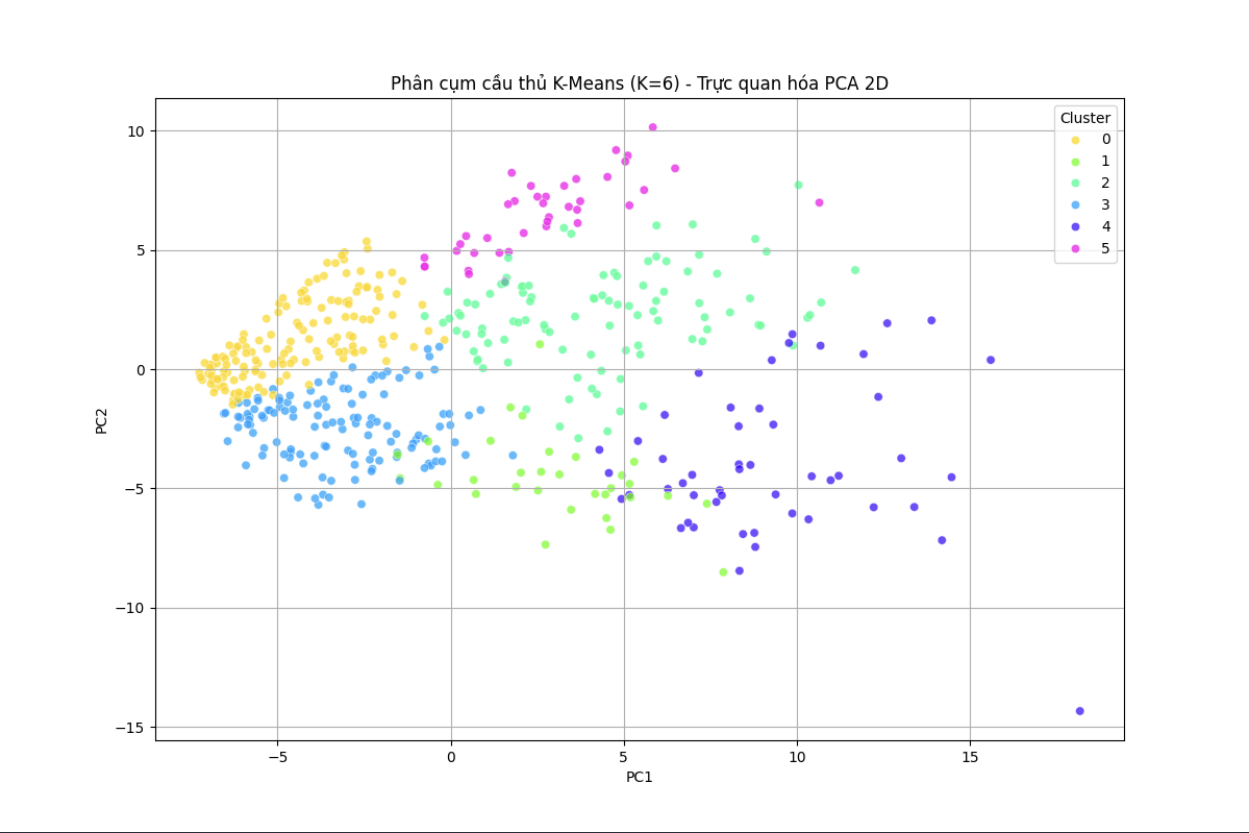
\includegraphics[width=\textwidth]{pca_kmeans.png}
    \caption{K-Means Player Clustering (K=6) - 2D PCA Visualization.}
    \label{fig:pca_kmeans_viz}
\end{figure}

\textbf{Remarks on the PCA plot:}
Proportion of variance explained by the 2 principal components (PC1 and PC2): 0.6499 (i.e., 64.99\%).
This indicates that the first two principal components explain approximately 65\% of the total variance in the data, with the remaining 35\% of information residing in other components.
The plot shows that the clusters are quite clearly divided, but there are some overlapping regions between clusters, especially in the central area (near the intersection of PC1 = 0, PC2 = 0).
This suggests that some players have relatively similar characteristics across clusters, possibly because their statistical parameters (e.g., number of goals, assists, or defensive indicators) do not differ significantly.
\begin{itemize}
    \item Cluster 0 (yellow) is mainly concentrated in the upper-left corner of the plot (negative PC1, positive PC2), possibly representing a group of players with distinct characteristics (e.g., defenders or goalkeepers, based on CSV data, as they tend not to score and are heavily involved in defense).
    \item Cluster 1 (light green) is located in the lower-right (positive PC1, negative PC2), possibly a group of forwards or attacking players who score many goals (like Alexander Isak, Yoane Wissa in this cluster).
    \item Cluster 2 (blue) is widely distributed in the central and right areas, possibly midfielders or full-backs with a balanced role between attack and defense (like Alexis Mac Allister, Andrew Robertson).
    \item Cluster 3 (light blue) is concentrated in the lower-left corner (negative PC1, negative PC2), possibly young or reserve players with little playing time and minimal contribution to attacking statistics (like Abdul Fatawu Issahaku, Adam Lallana).
    \item Cluster 4 (purple) is located on the right side (positive PC1), possibly attacking players or wingers with many dribbles and attacking involvement (like Alejandro Garnacho, Adama Traoré).
    \item Cluster 5 (pink) is scattered but concentrated in the region of large positive PC2, possibly center-backs or defensive players with high defensive stats (like Virgil van Dijk, Wout Faes).
\end{itemize}

\subsection{Conclusion} % Tài liệu gốc có 3.3.4.
The \texttt{pca\_visual\_kmeans.py} script successfully fulfills the requirement of visualizing K-Means player clustering results by using PCA to reduce data dimensionality to 2D.
The result is a 2D scatter plot and a new dataset accompanied by PCA coordinates, allowing for an initial visual assessment of cluster separation.
Although this method has certain limitations related to information loss, it remains a useful tool in the data analysis toolkit for exploring and presenting clustering results in a more understandable way.
% End of Chapter 3

% Chương 4
\chapter{Collecting Transfer Values and Building a Player Value Estimation Model}

\section{Collecting and Processing Player Transfer Values for the 2024-2025 Season}

\subsection{Introduction}
This report section presents the process of collecting football player transfer value data for the 2024-2025 season from the website \url{https://www.footballtransfers.com}.
This process focuses on obtaining information for players with actual playing time exceeding 900 minutes, based on the provided data.
The main source code file is \texttt{transfer\_values\_2024-2025.py}.

\subsection{Directory Structure and Libraries Used}
\begin{itemize}
    \item Directory structure: Organized with the main code file \texttt{transfer\_values\_2024-2025.py} and the configuration file \texttt{config.json} in the root directory.
    \item Input data is sourced from the \texttt{../problem\_1/} directory, and results are saved in the \texttt{OUTPUT/} directory (including \texttt{raw\_data.csv}, \texttt{player\_transfer\_values.csv}, \texttt{estimation\_data.csv}).
    \item {Main libraries used:} Python, \texttt{os}, \texttt{re}, \texttt{time}, \texttt{pandas}, \texttt{json}, \texttt{BeautifulSoup} (from \texttt{bs4}), and \texttt{selenium} (along with its submodules).
\end{itemize}

\subsection{Execution Process}
\begin{enumerate}[label=\textbf{Step \arabic*:}, leftmargin=* , itemsep=1ex]
    \item \textbf{Load Configuration} \\
    The script begins by loading configuration parameters from the \texttt{config.json} file via the \texttt{load\_config} function.
    This file contains important paths (e.g., \texttt{paths.part1\_results\_relative} for the playing time data file, \texttt{paths.output\_folder} for the results directory), the target URL (\texttt{scraping.transfer\_url}), user-agent information (\texttt{scraping.user\_agent} to simulate a browser), CSS selectors (in \texttt{selectors}) to locate specific data snippets on the webpage (such as player name, ETV, "Next page" button), and the minimum playing time threshold (\texttt{processing.min\_minutes\_threshold}).

    \item \textbf{Data Collection (Web Scraping) - performed in the \texttt{scrape\_transfer\_data} function:}
    \begin{itemize}[leftmargin=0em]
        \item The \texttt{scrape\_transfer\_data} function uses Selenium to open the URL of the player list page (e.g., Premier League) specified in \texttt{config.json}.
        \item The script iterates through each page in the player list.
        \item Selenium waits for essential page elements, such as the player data table (\texttt{selectors.player\_table}), to load completely before proceeding with extraction.
        \item For each player (each \texttt{selectors.player\_row} row in the table), the following information is extracted based on CSS selectors defined in \texttt{config.json}:
        \begin{itemize}
            \item Player name (\texttt{selectors.player\_name})
            \item Team name (\texttt{selectors.team\_name})
            \item Estimated Transfer Value (ETV - \texttt{selectors.etv})
            \item Age (\texttt{selectors.age})
            \item Position (\texttt{selectors.position})
            \item Skill (\texttt{selectors.skill})
            \item Potential (\texttt{selectors.potential})
        \end{itemize}
        \item Processing transfer value (ETV) immediately upon collection: Raw ETV data (e.g., "€50.5m") is cleaned and converted to millions of Euros at this step using the \texttt{clean\_transfer\_value} function. This function:
        \begin{itemize}
            \item Removes currency symbols (e.g., '€', '\$') and commas.
            \item Identifies and processes 'm' (million) or 'k' (thousand) suffixes to convert to the full numeric value.
            \item Standardizes the value to millions (e.g., 50.5).
            \item If the value is invalid, it returns \texttt{None}.
        \end{itemize}
        \item Similarly, other numeric values like Age, Skill, Potential are extracted as text, and the \texttt{safe\_get\_numeric} function attempts to convert them to numeric form, handling commas if present.
        \item "Button Clicking" Mechanism (Pagination):
        \begin{itemize}
            \item After processing all players on a page, the script looks for the "Next page" button.
            \item The \texttt{get\_next\_page\_button} function is called, using \texttt{WebDriverWait} to wait up to 5 seconds for the "Next page" button (identified by the \texttt{selectors.next\_page\_enabled} selector from \texttt{config.json}, e.g., \texttt{button.pagination\_next\_button:not([disabled])}) to become available and clickable. This selector ensures only an active button is selected.
            \item If a valid "Next page" button is not found (e.g., on the last page or due to a page load error), \texttt{get\_next\_page\_button} returns \texttt{None}, and the data collection loop across pages will terminate.
            \item If the button is found:
            \begin{itemize}
                \item The script executes \sloppypar
                \texttt{driver.execute\_script("arguments[0].scrollIntoView(\{block: 'center'\});", next\_btn)} to scroll the button into the center of the browser's viewport. This minimizes the risk of the button being obscured by other elements and becoming unclickable.
                \item A short random pause \sloppypar
                (\texttt{time.sleep(random.uniform(0.4, 0.8))}) is applied.
                \item The script attempts to click the button using \texttt{next\_btn.click()}. If an \sloppypar
                \texttt{ElementClickInterceptedException} \sloppypar (meaning another element is obscuring the button), the script switches to a fallback: performing the click via JavaScript with \texttt{driver.execute\_script("arguments[0].click();", next\_btn)}.
                \item After a successful click, a longer pause (\texttt{time.sleep(random.uniform(2.0, 3.5))}) is applied to wait for the new page to load completely before continuing the loop.
            \end{itemize}
        \end{itemize}
        \item After the \texttt{scrape\_transfer\_data} function completes iterating through all pages and collecting player information into a temporary data structure (a Python dictionary), this entire data block (\texttt{scraped\_data}) will be passed to the next processing step, where it will be converted into a DataFrame and saved as a raw data file (\texttt{raw\_data.csv}).
    \end{itemize}

    \item \textbf{Filter data based on playing time:}
    This is a core step to ensure only players meeting the playing time criteria are retained.
    \begin{itemize}[leftmargin=0em]
        \item \textbf{Get list of valid players (\texttt{get\_valid\_players\_from\_part1}):} This function reads the external CSV file \texttt{results1.csv} (path declared in \texttt{config.json} via the key \texttt{paths.part1\_results\_relative}).
        \item From this \texttt{results1.csv} file, the script will primarily use two important columns to filter players:
        \begin{itemize}
            \item The column containing player names, identified by the value of the \newline
            \texttt{processing.part1\_player\_column} key in \texttt{config.json} (e.g., "Name").
            \item The column containing player playing time, identified by the value of the \texttt{processing.part1\_minutes\_column} key in \texttt{config.json} (e.g., "Playing Time: minutes").
        \end{itemize}
        \item Subsequently, the playing time from this column will be converted to a numeric type and compared with the \texttt{min\_minutes\_threshold} (900 minutes) to generate a list of "valid" player names.
    \end{itemize}

    \item \textbf{Apply filter to collected data}
    \begin{itemize}
        \item In the \texttt{process\_transfer\_data} function, if the list of valid players \newline 
        (\texttt{valid\_player\_set}) is not empty, the script will proceed with filtering.
        \item A temporary column \texttt{Player\_Normalized} is created in \texttt{df\_raw} by normalizing the 'Player' column (removing excess whitespace).
        \item \texttt{df\_raw} is then filtered to retain only rows where the value in the \newline \texttt{Player\_Normalized} column is present in \texttt{valid\_player\_set}.
        \item The temporary \texttt{Player\_Normalized} column is deleted after filtering.
        \item If no list of valid players is found from the input CSV file (e.g., file does not exist, no players meet the threshold), then \texttt{df\_raw} (data not yet filtered by playing time) will be returned.
    \end{itemize}
\end{enumerate}

\subsection{Results}

\begin{figure}[H]
    \centering
    % Thay 'player_transfer_values_example.png' bằng tên file ảnh thực tế của bạn
    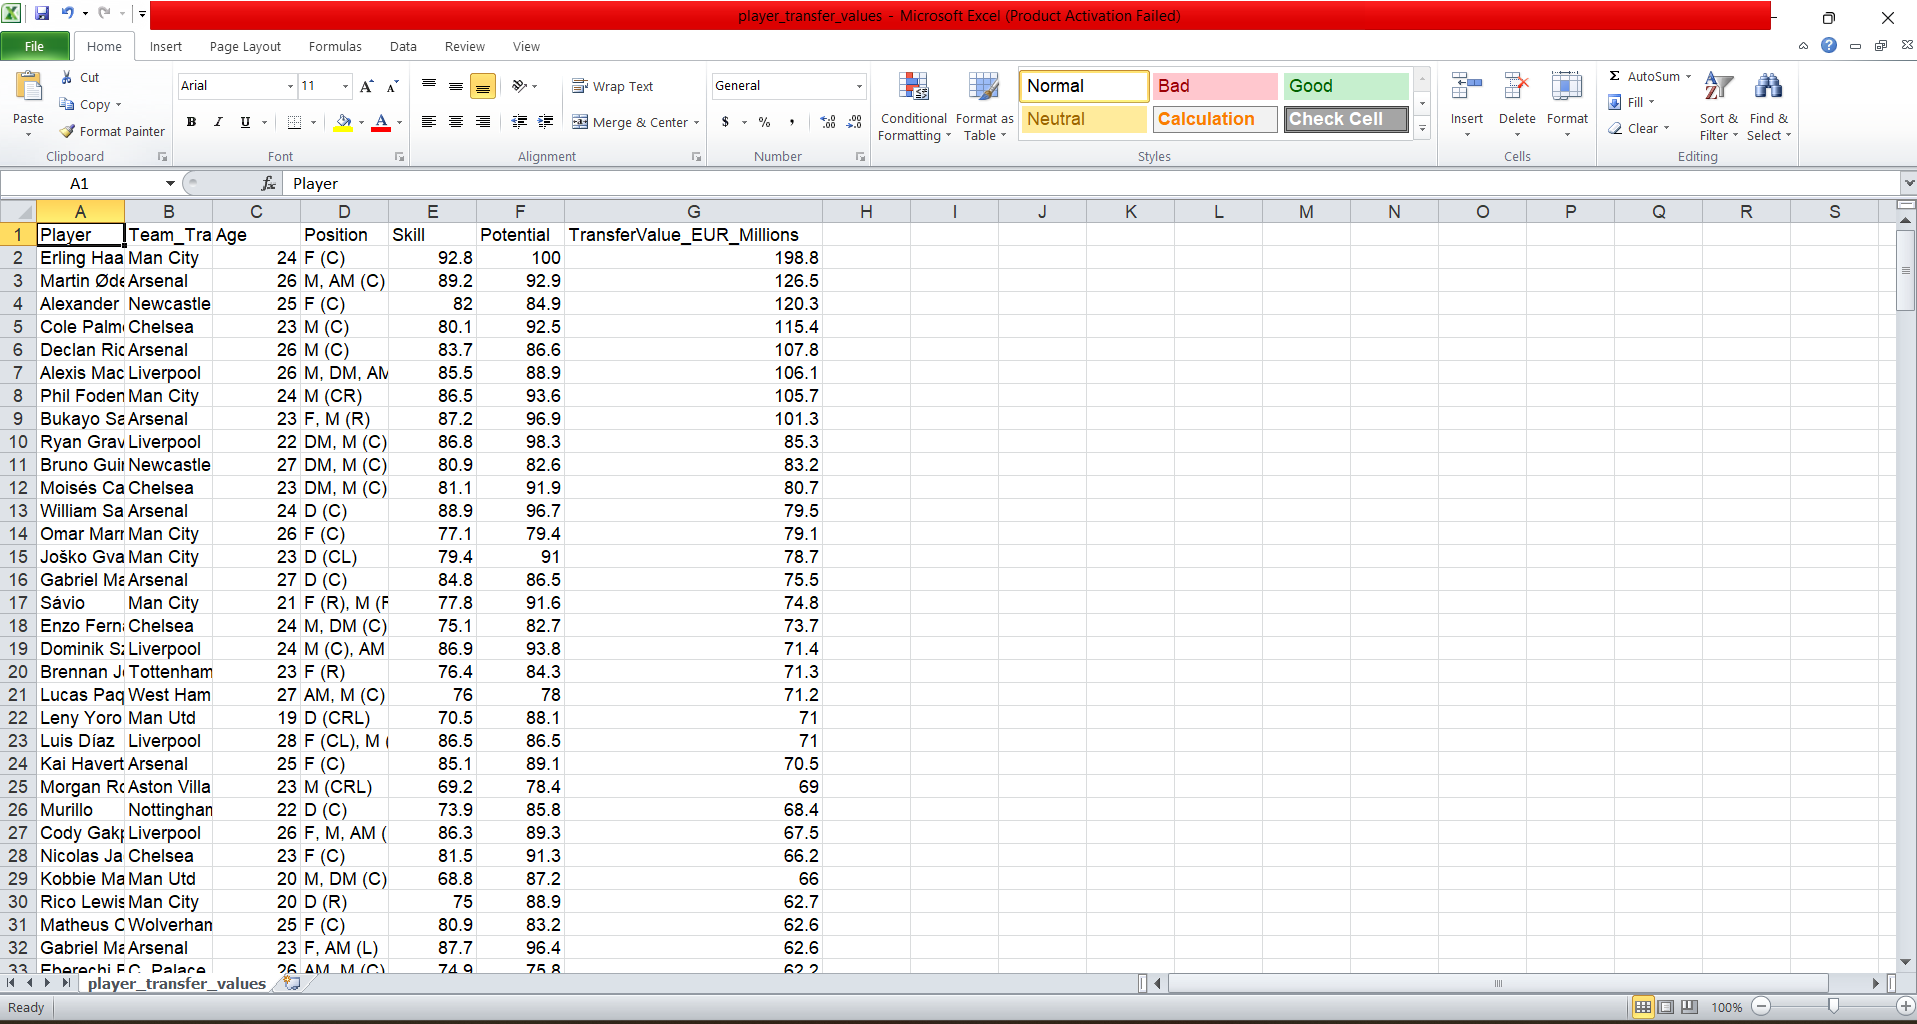
\includegraphics[width=\textwidth]{player_values.png}
    \caption{Example of player transfer value data after processing.}
    \label{fig:player_transfer_values}
\end{figure}

The automated data collection and processing workflow has been successfully implemented through the \texttt{transfer\_values\_2024-2025.py} script and the \texttt{config.json} configuration file.
The result of this process is the collection and filtering of detailed information for \textbf{284 players} with actual playing time exceeding 900 minutes in the 2024-2025 season from \texttt{footballtransfers.com}.
The data obtained for each player includes the following important indicators:
\begin{itemize}
    \item Team
    \item Age
    \item Position
    \item Skill
    \item Potential
    \item Estimated Transfer Value (TransferValue\_EUR\_Millions)
\end{itemize}
All this data has been stored in output files via the \texttt{save\_data} function:
\begin{itemize}
    \item \texttt{player\_transfer\_values.csv}: final data on player transfer values, processed and filtered
    \item \texttt{estimation\_data.csv}: prepared for use in the next section: predicting player values
\end{itemize}

\section{Building a Football Player Value Estimation Model}

\subsection{Introduction}
The football player transfer market is a complex and dynamic field where accurately valuing players plays a crucial role for clubs.
This report section presents a method for building a machine learning model to estimate player transfer values, based on performance statistics, potential, and other factors.
The objective is to propose a systematic process from data collection, feature engineering, model selection to evaluation and interpretation of results.
The target variable is the player's transfer value, transformed using a logarithmic function (\texttt{Log\_TransferValue}) to stabilize variance and reduce the impact of outliers.

\subsection{Data Description and Preprocessing}
\subsubsection*{Data Sources and Merging}
\begin{itemize}
    \item \textbf{Data Sources:}
    \begin{itemize}
        \item Estimation data (\texttt{estimation\_data.csv}): Contains basic information and some initial player indicators.
        \item Results data (\texttt{results1.csv}): May contain more detailed performance indicators from another source.
    \end{itemize}
    \item \textbf{Data Merging:}
    \begin{itemize}
        \item The two datasets are merged based on player and team information.
        \item Team names have been standardized to ensure accurate merging (e.g., "B'mouth" to "Bournemouth").
    \end{itemize}
    \item \textbf{Result after merging:} (283, 85), meaning 283 samples (players) and 85 initial features. This is performed in the \texttt{load\_and\_merge\_data} function.
\end{itemize}

\subsubsection*{Feature Engineering}

The goal of feature engineering is to create more meaningful new variables from raw data, helping the model learn better. Key steps include:
\begin{itemize}
    \item \textbf{Create Primary Position (PrimaryPosition):} From the \texttt{Position\_x} column (which may contain multiple positions), only the first position is taken as the player's primary position. Missing or undefined values are assigned as 'Unknown'.
    \item \textbf{Standardize and convert numeric data types:} Columns like 'Skill', 'Potential', 'Age\_x', 'Expected: expected goals (xG)', 'Expected: expected Assist Goals (xAG)', 'TransferValue\_EUR\_Millions' are converted to numeric types. Conversion errors (if any) are handled by assigning \texttt{NaN}.
    \item \textbf{Calculate performance metrics per 90 minutes:}
    \begin{itemize}
        \item \texttt{GoalContrib\_per90}: Total goals and assists per 90 minutes.
        \item \texttt{DefensiveActions\_per90}: Total successful tackles (TklW) and interceptions (Int) per 90 minutes.
        \item \texttt{Progression\_per90}: Total progressive carries and passes per 90 minutes.
    \end{itemize}
    \item \textbf{Standardize percentage columns:} Columns like 'Total: Pass completion (Cmp\%)', 'Aerial Duels: Won\%' are converted from string format (e.g., "85\%") to decimal format (e.g., 0.85).
    \item \textbf{Transform target variable:}
    \begin{itemize}
        \item Transfer value ('TransferValue\_EUR\_Millions') is ensured to be non-negative (negative values are clipped to 0).
        \item Create the \texttt{Log\_TransferValue} column by applying the \texttt{np.log1p} function (natural logarithm of 1+x) to \texttt{TransferValue\_EUR\_Millions}. This transformation helps to:
        \begin{itemize}
            \item Reduce the skewness of the transfer value distribution.
            \item Stabilize variance.
            \item Ensure the input to the logarithm function is always positive, even if the transfer value is 0.
        \end{itemize}
    \end{itemize}
    \item \textbf{Result after feature engineering:} (283, 90), indicating that 5 new features were created or columns were processed. This process is performed in the \texttt{advanced\_feature\_engineering} function.
\end{itemize}

\subsection{Feature Selection and Data Preparation for the Model}
\subsubsection{Feature Selection}

Not all created features are useful for the model. The following features were selected for inclusion in the model:
'Skill',
'Potential',
'Age\_x',
'GoalContrib\_per90',
'DefensiveActions\_per90',
'Progression\_per90',
'Expected: expected goals (xG)',
'Expected: expected Assist Goals (xAG)',
'Total: Pass completion (Cmp\%)',
'Aerial Duels: Won\%',
'PrimaryPosition\_enc'.

\textbf{Reasons for selection (inferred from feature names and general knowledge):}
\begin{itemize}
    \item \textit{Individual attributes:} 'Age\_x', 'Skill', and 'Potential' are fundamental indicators assessing a player's current quality, experience, and future development potential. Age is a crucial factor, often having a non-linear relationship with player value.
    \item \textit{Attacking performance:} 'GoalContrib\_per90', 'Expected: expected goals (xG)', 'Expected: expected Assist Goals (xAG)' measure the ability to contribute directly to the attack.
    \item \textit{Defensive performance:} 'DefensiveActions\_per90' reflects contributions in defense.
    \item \textit{Ball progression and control ability:} 'Progression\_per90' and 'Total: Pass completion (Cmp\%)' indicate ball handling and distribution skills.
    \item \textit{Specific physical/skill attributes:} 'Aerial Duels: Won\%' is important for certain positions.
    \item \textit{Positional factor:} 'PrimaryPosition' is an important factor as player values often differ significantly between positions.
\end{itemize}

\subsubsection{Data Preparation}

Final data preparation steps before model input, performed in the \texttt{prepare\_model\_data} function:
\begin{itemize}
    \item \textbf{Handle Missing Values:} For selected numeric features, missing values are imputed with the mean of that column.
    \item \textbf{Numerical Feature Scaling:} Numeric features are standardized using \texttt{StandardScaler} (subtracting the mean and dividing by the standard deviation to achieve a mean of 0 and variance of 1). This helps scale-sensitive algorithms (like XGBoost when not using \texttt{tree\_method='hist'} or distance-based models) perform more effectively.
    \item \textbf{Categorical Feature Encoding:} The \texttt{PrimaryPosition} feature is encoded using \texttt{LabelEncoder}. Each unique position will be assigned an integer value.
    \item \textbf{Create feature matrix (X) and target vector (y):}
    \begin{itemize}
        \item X: Matrix containing processed features (standardized and encoded). Dimensions: (283, 10).
        \item y: Vector containing the target variable \texttt{Log\_TransferValue}. Dimensions: (283,).
    \end{itemize}
    \item \textbf{Data check:} Ensure the X matrix is not empty and the number of samples in X matches y.
\end{itemize}

\subsection{Model Selection and Training}
\subsubsection{Model Selection}

The model selected for estimating player value is XGBoost (Extreme Gradient Boosting).
\textbf{Reasons for choosing the XGBoost model to estimate player value:}
\begin{itemize}
    \item \textit{Ability to capture complex and non-linear relationships:} Player value is determined by the multidimensional interaction of many factors such as age, skill, potential, and performance. XGBoost, with its structure based on an ensemble of decision trees, excels at automatically detecting and modeling these complex relationships (e.g., the effect of age is not always linear, or potential has different values at different ages) without requiring pre-definition. This is extremely important for accurately reflecting the nature of player valuation.
    \item \textit{Superior predictive performance and effective overfitting control:} XGBoost is renowned for its ability to achieve high accuracy on tabular data. This algorithm integrates regularization mechanisms (L1, L2) and optimization techniques (such as \texttt{early\_stopping\_rounds} used here) that help prevent the model from becoming overly complex or "memorizing" the training data. As a result, the model has better generalization capabilities on new data, ensuring the reliability of player value predictions.
    \item \textit{Efficient optimization and feature interpretability:} XGBoost is designed for rapid training, even on relatively large datasets, thanks to techniques like parallel processing and the histogram-based method (\texttt{tree\_method='hist'}). More importantly, it provides detailed information about the importance of each feature (e.g., \texttt{Age\_x}, \texttt{Skill}, \texttt{GoalContrib\_per90}), allowing us to understand which factors have the greatest impact on valuation. This not only helps in evaluating the model but also provides valuable insights for football analysts and managers.
\end{itemize}

\subsubsection{Training and Hyperparameter Optimization}

The training process is performed in the \texttt{train\_model} function:
\begin{itemize}
    \item \textbf{Data Splitting:} The data (X, y) is split into a training set and a test set with an 80:20 ratio (\texttt{test\_size=0.2}). \texttt{X\_train} has dimensions (226,11).
    \item \textbf{Hyperparameter Tuning:}
    \begin{itemize}
        \item Uses \texttt{RandomizedSearchCV} to find the best set of hyperparameters for XGBoost.
        \item \texttt{RandomizedSearchCV} tests a number of random parameter combinations (\texttt{n\_iter=20}) from a predefined search space (\texttt{param\_grid}).
        \item Cross-validation with \texttt{cv=5} is used during the search process to ensure the stability of the results.
        \item The evaluation metric used during the search is \texttt{r2} (R-squared).
    \end{itemize}
    \item \textbf{Best hyperparameters found:}
    \begin{itemize}
        \item subsample: 0.6
        \item n\_estimators: 1000
        \item max\_depth: 6
        \item learning\_rate: 0.05
        \item gamma: 0.5
        \item colsample\_bytree: 0.6
    \end{itemize}
    \item \textbf{Final Model Training:} The XGBoost model is retrained on the entire training set (\texttt{X\_train}, \texttt{y\_train}) with the best hyperparameters just found. \texttt{early\_stopping\_rounds=50} and \texttt{eval\_set=[(X\_test, y\_test)]} are used to monitor performance on the test set and stop early if there is no improvement, to avoid overfitting.
    \item \textbf{Training Environment:} The XGBoost model training process is performed on a CPU.
\end{itemize}

\subsection{Model Evaluation}

The model is evaluated on the entire processed dataset (X, y).
\begin{itemize}
    \item \textbf{R² score (Coefficient of Determination R-squared = 0.880):} This means that approximately 88.0\% of the variance in \texttt{Log\_TransferValue} can be explained by the model's input features. This is a fairly good result, indicating the model's ability to capture important factors influencing player value.
    \item \textbf{MSE (Mean Squared Error = 0.088):} This is the average of the squared differences between the predicted and actual values (on a logarithmic scale). A smaller MSE value is better.
\end{itemize}

\subsection{Analysis and Visualization of Results}

Visualizations help to better understand the model's performance and internal workings.

\subsubsection*{Actual vs. Predicted Values Plot (\texttt{actual\_vs\_predicted.png})}
\begin{figure}[H]
    \centering
    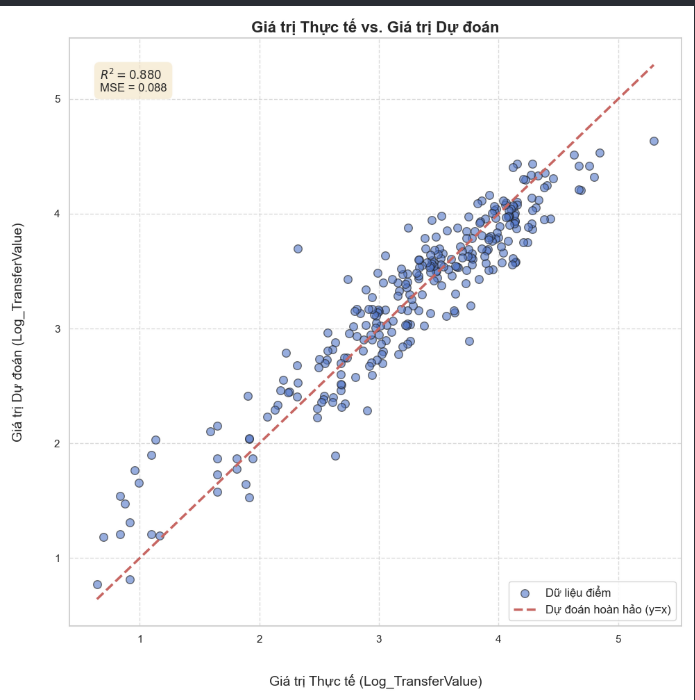
\includegraphics[width=\textwidth]{actual_vs_predicted.png}
    \caption{Actual vs. Predicted Values Plot.}
    \label{fig:actual_vs_predicted}
\end{figure}

Based on the plot: The model predicts player values \textbf{quite well}, as shown by data points concentrated relatively close to the diagonal line (perfect prediction) and a high R² score (0.880).
However, the model \textbf{still has errors} (MSE = 0.088, on a log scale), with some predictions deviating significantly from actual values, particularly noticeable at the lower and higher value ranges.

\subsubsection*{Residual Plot (\texttt{residual\_plot.png})}
\begin{figure}[H]
    \centering
    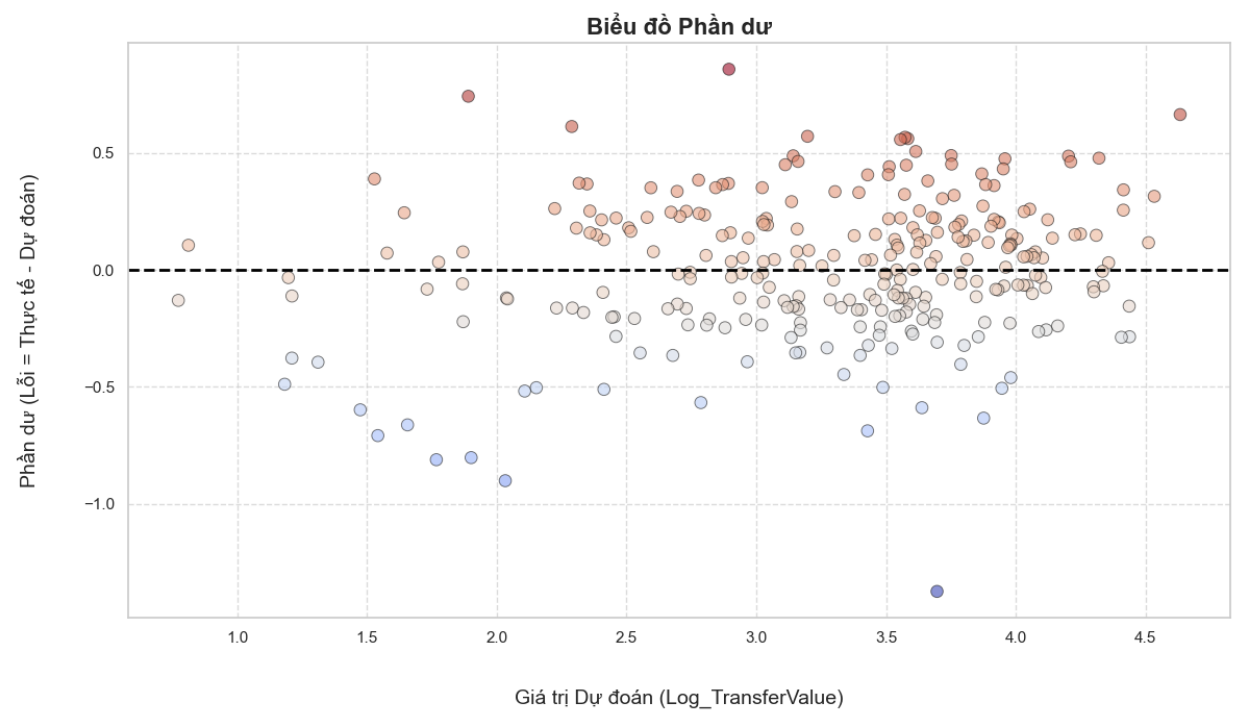
\includegraphics[width=\textwidth]{residual_plot.png}
    \caption{Residual Plot.}
    \label{fig:residual_plot}
\end{figure}

The residual plot shows that most points are distributed near the 0 line on the Residual axis, with a few points deviating significantly, especially at high predicted values (large \texttt{Log\_TransferValue}).
This indicates that the XGBoost model performs well in predicting player values, with high accuracy for the majority of the data, but may need improvement for outliers or high-value cases.

\subsubsection*{XGBoost Feature Importance (\texttt{xgb\_feature\_importance.png})}
\begin{figure}[H]
    \centering
    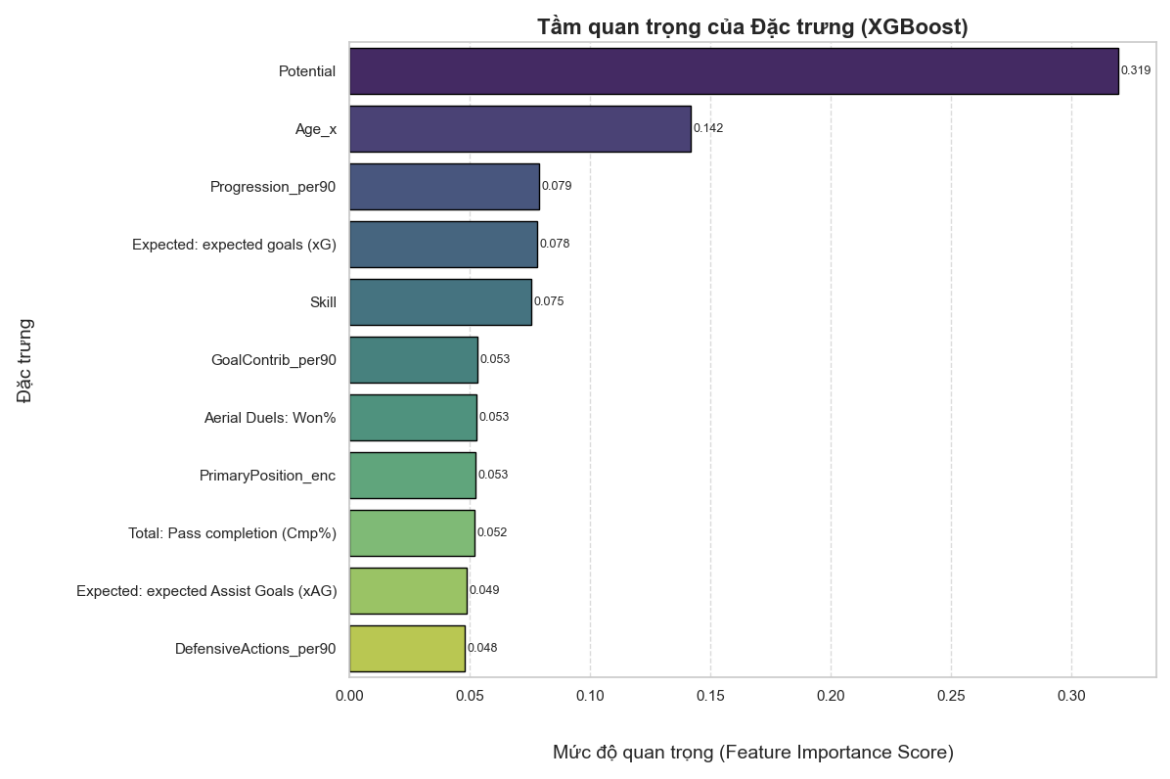
\includegraphics[width=\textwidth]{xgb_feature_importance.png}
    \caption{Feature Importance Plot (XGBoost).}
    \label{fig:xgb_feature_importance}
\end{figure}

The XGBoost Feature Importance plot shows "Potential" as the most important feature with a score of 0.319, followed by "Age" (0.142).
Features like "Progression\_per90" (0.079), "Expected: expected goals (xG)" (0.078), and "Skill" (0.075) also have a significant impact.
Other features such as "DefensiveActions\_per90" (0.048) have a lower level of importance.
This indicates that the model relies heavily on player potential and age, while also considering performance indicators like progression and skill.

\subsection{Conclusion and Future Development}
\subsubsection*{Conclusion}
The proposed method successfully built an XGBoost model to estimate player value (log-transformed) with fairly good performance (R2=0.880). This process included crucial steps from data merging, feature engineering, feature selection and preparation, to model training, optimization, and evaluation. Selected features such as \texttt{Skill}, \texttt{Potential}, \texttt{Age}, attacking/defensive performance metrics per 90 minutes, and passing/aerial duel statistics demonstrated their contribution to value prediction. The use of \texttt{RandomizedSearchCV} helped find good hyperparameters for XGBoost. Visualizations provided insightful interpretations of the model's behavior.

\subsubsection*{Future Development}
\begin{itemize}
    \item \textbf{Evaluation on an independent test set:} To obtain a more objective assessment of generalization ability, the model needs to be evaluated on a completely separate test dataset (not used during hyperparameter optimization).
    \item \textbf{Experiment with other models:} Compare XGBoost with other algorithms like LightGBM, CatBoost, or simple neural network models.
    \item \textbf{More advanced feature engineering:}
    \begin{itemize}
        \item Consider interactions between features (e.g., \texttt{Skill} * \texttt{GoalContrib\_per90}).
        \item Collect more data (e.g., league information, contract details, team achievements).
    \end{itemize}
    \item \textbf{Detailed error analysis:} Examine cases where the model predicts most inaccurately to better understand its limitations.
    \item \textbf{Address data imbalance issues (if any):} If player values are very unevenly distributed, imbalance handling techniques may be needed.
    \item \textbf{Periodic model updates:} Player values and influencing factors change over time, so the model needs to be retrained and updated periodically with new data.
\end{itemize}
% Hết chương 4


\begin{thebibliography}{99}
\bibitem{XGBoostDocs}
XGBoost Developers. (2024). \textit{XGBoost Documentation (Release 3.0.0)}.
Accessed on May 5, 2025, from \url{https://xgboost.readthedocs.io/en/release_3.0.0/}

\bibitem{OngXuanHongBlogXGBoost}
Ông Xuân Hồng (2017, December 21). \textit{XGBoost – the algorithm that wins many Kaggle competitions}.
Accessed on May 5, 2025, from \url{https://ongxuanhong.wordpress.com/2017/12/21/xgboost-thuat-toan-gianh-chien-thang-tai-nhieu-cuoc-thi-kaggle/}

\bibitem{Li2022MLValue}
Li, C., Kampakis, S., \& Treleaven, P. (2022). \textit{Machine Learning Modeling to Evaluate the Value of Football Players}.
arXiv preprint arXiv:2207.11361. Accessed on May 5, 2025, from \url{https://arxiv.org/pdf/2207.11361.pdf}

\end{thebibliography}
\end{document}